
\documentclass[twoside,a4paper,11pt]{article} % double-sided
%---------------------------------------------------------------------------------------------------------------------------------

\usepackage{a4} % gives a4 paper format 
\usepackage{hyperref}

%%% Math symbols and fonts packages
\usepackage{latexsym} % symbol and maths package
\usepackage{amsmath} % symbol and maths package
\usepackage{xspace}  % useful for macro definitions

%%% Layout 
\usepackage{fancyhdr} % for header and footer on pages
\usepackage{float} % for graphics/including pictures
\usepackage{listings}% very useful aid for including computer code in the document
\usepackage{enumerate}% useful add on for numbered lists
\usepackage{enumitem} % lets me use itemsep for enumeration .. 

%%% Layout Aids [specifically json files, adding some bells]
\lstdefinelanguage{json}{
    basicstyle=\normalfont\ttfamily,
    numbers=left,
    numberstyle=\scriptsize,
    stepnumber=1,
    numbersep=8pt,
    showstringspaces=false,
}
\lstdefinelanguage{java}{
  showspaces=false,
  showtabs=false,
  breaklines=true,
  showstringspaces=false,
  breakatwhitespace=true,
  commentstyle=\color{pgreen},
  keywordstyle=\color{pblue},
  stringstyle=\color{pred},
  basicstyle=\ttfamily,
  moredelim=[il][\textcolor{pgrey}]{$$},
  moredelim=[is][\textcolor{pgrey}]{\%\%}{\%\%}
}


%%% Graphics
\usepackage{pdfsync} % for source specials directly in pdf, fixed prob below. 
\usepackage[pdftex]{graphicx,xcolor}
%\graphicspath{ {images/} } %I'll use this when we have more images to store in it's own directory, causes problems? ->pdfsync 
\usepackage{pgf,tikz,cite}

%%% CHANGE THE PAGE LAYOUT 
\addtolength{\textwidth}{0.5cm} % adds 0.5cm to textwidth:
\addtolength{\evensidemargin}{-0.53cm} % Keep the text centered, make the margin of all even-numbered pages 0.53cm smaller
\addtolength{\oddsidemargin}{-0.15cm} % make the margin of all odd-numbered pages 0.15cm smaller

%%% MACROS
% I like this macro, it makes indenting easier, solves the viewing problem for double sided pages 
\newlength\tindent 
\setlength{\tindent}{\parindent}
\setlength{\parindent}{0pt}
\renewcommand{\indent}{\hspace*{\tindent}}


%---------------------------------------------------------------------------------------------------------------------------------
%%% The document actually starts here
\begin{document}
\nocite{*}

%%% Produces the title page
% Start by centering it all 
% write text headers 
% minipages for the seperation for auth and sup.  
\begin{titlepage}
  \center
  \textsc{\Large Kings College London}\\[1.5cm] 
  \textsc{\Large 7CCSMGPR}\\[0.5cm] 
  \textsc{\large Final Report}\\[0.5cm] 
  \textbf{\LARGE Traffic Simulation}\\[1.5cm] 

%------------------  
  \begin{minipage}{0.5\textwidth} %0.5 seems to work nice 
    \begin{flushleft} \large
      \emph{Group Members:}\\
      Iordanis Paschalidis\
      \\Rolando A. Vicente Villalta\
      \\Seyed M. Yamoot\
      \\Orkhan Seyidov\
      \\Anthony Tsiopoulos
    \end{flushleft}
  \end{minipage}
  \begin{minipage}{0.4\textwidth}
    \begin{flushright} \large
      \emph{Professor:}\\ 
      Dr. Laurence Tratt
    \end{flushright}
  \end{minipage}\\[3cm] 
  
  \textsc{\large \today} 
  \thispagestyle{empty} % suppress page number
    
\end{titlepage}

%---------------------------
%%% ABSTRACT 
% Since this is not a completed piece of work, we will leave out the abstract. 
% We could use it to define the problem domain, but let's assume (?) the reader is aware. 
\begin{abstract}
In this project we have designed and implemented a novel method for the animation and synthesis of the real life scenario of the traffic management on a large scale network. Our method adapts the agent based technique where the vehicle have the ability to make turns and change speed, stop and start independent of the map type. We have created a user interaction where the user has the ability to change the parameters of the system operation such changing the number vehicle and speed. Furthermore our simulation model is preformed on multiple map putting into consideration the traffic management and traffic policy.   
\end{abstract}
\thispagestyle{empty} % suppresses page number


%-----------------------------------------------------------------------------------------------------------------------------
\newpage  
%%% TOC
\tableofcontents
\thispagestyle{empty} % Use this again here, otherwise the page starts on TOC 


%------------------------------------------------------------------------------------------------------------------------------
\newpage
%%% SECTIONS OF MAIN PAPER
\setcounter{page}{1} %
%**sigh** lolled hard. Fixed issue. Now clean then erase when clean is accomplished. **sigh**
% Using \input{} instead of \include{} to avoid pagebreaks 

\section{Introduction}

\subsection{Overview}

As the population increases the traffic management is becoming more complex and challenging in various urban areas around the world.  This high demand of traffic management required a modelling, simulation and observation of the traffic flow and being able to monitor the effect of traffic congestion and incidences to study the effectiveness of the signs, hardware devices such as traffic lights and other barriers that are used to manage and improve the traffic policies and guild-lines related to the traffic management regulation, and also being able to assist the design and development of roads, junctions and highways.\newline

One of the effective tools used in order to overcome the high demand of population and being able to analyse a wide range of dynamic problem associated with complex scenarios which cannot be described in an analytical approach is simulation modelling. These simulating models have been classified by the level of detailing and its interaction based on various system entities or component, which there interaction are complex in real world. these simulations models represent the dynamic behaviour in a mathematical and logical way in the system operation. Over the past six decades there has been significant improvement in design and development of the traffic simulation models in order to experiment the real world traffic operation there are various techniques and approaches used in implementation and design of these simulation models which   now days the use of these tool are necessary in order to analyse and examine the real world scenario of the traffic operation, which is a common tool used for traffic engineers. The following list are the main reason for the need of traffic simulation:

\begin{enumerate}
\item When we require to observe the behaviour of the vehicles and entitles of the system such as traffic signs and traffic lights in an animated way.
\item When there is an uncertainty in the mathematical analysis result.  
\item In instances where the analytical or mathematical modelling approach is inadequate or infeasible, this can be due to the complexity of the urban operation.
\end{enumerate}

In this project we have designed and developed a traffic simulation by animating the vehicle operation on a 2-Dimention map as shown in figure 1, where the vehicles can operate on single and multi-lane, on opposite directions. Our approach adapts the agent based-method where the vehicle detect their condition based on their position where the vehicle can stop or turn depending on their position. The user has the ability to change the parameters of the system such increasing and decreasing the numbers of cars, delay of the traffic light and flow-rate (frequency). The user has various map selection as shown, this can be either a single junction or multiple junction operation and the user has the ability to change the delay of the traffic light. In this project we have considered and adapted the traffic policies, such as implementing traffic lights in order to manage the traffic flow and designed various lanes and junction considering the road network operation. The system has a time control follow density operation, where the number of cars operating in the system increases to it maximum limit   as the time merges its peak time. \newline

\begin{figure}[H]
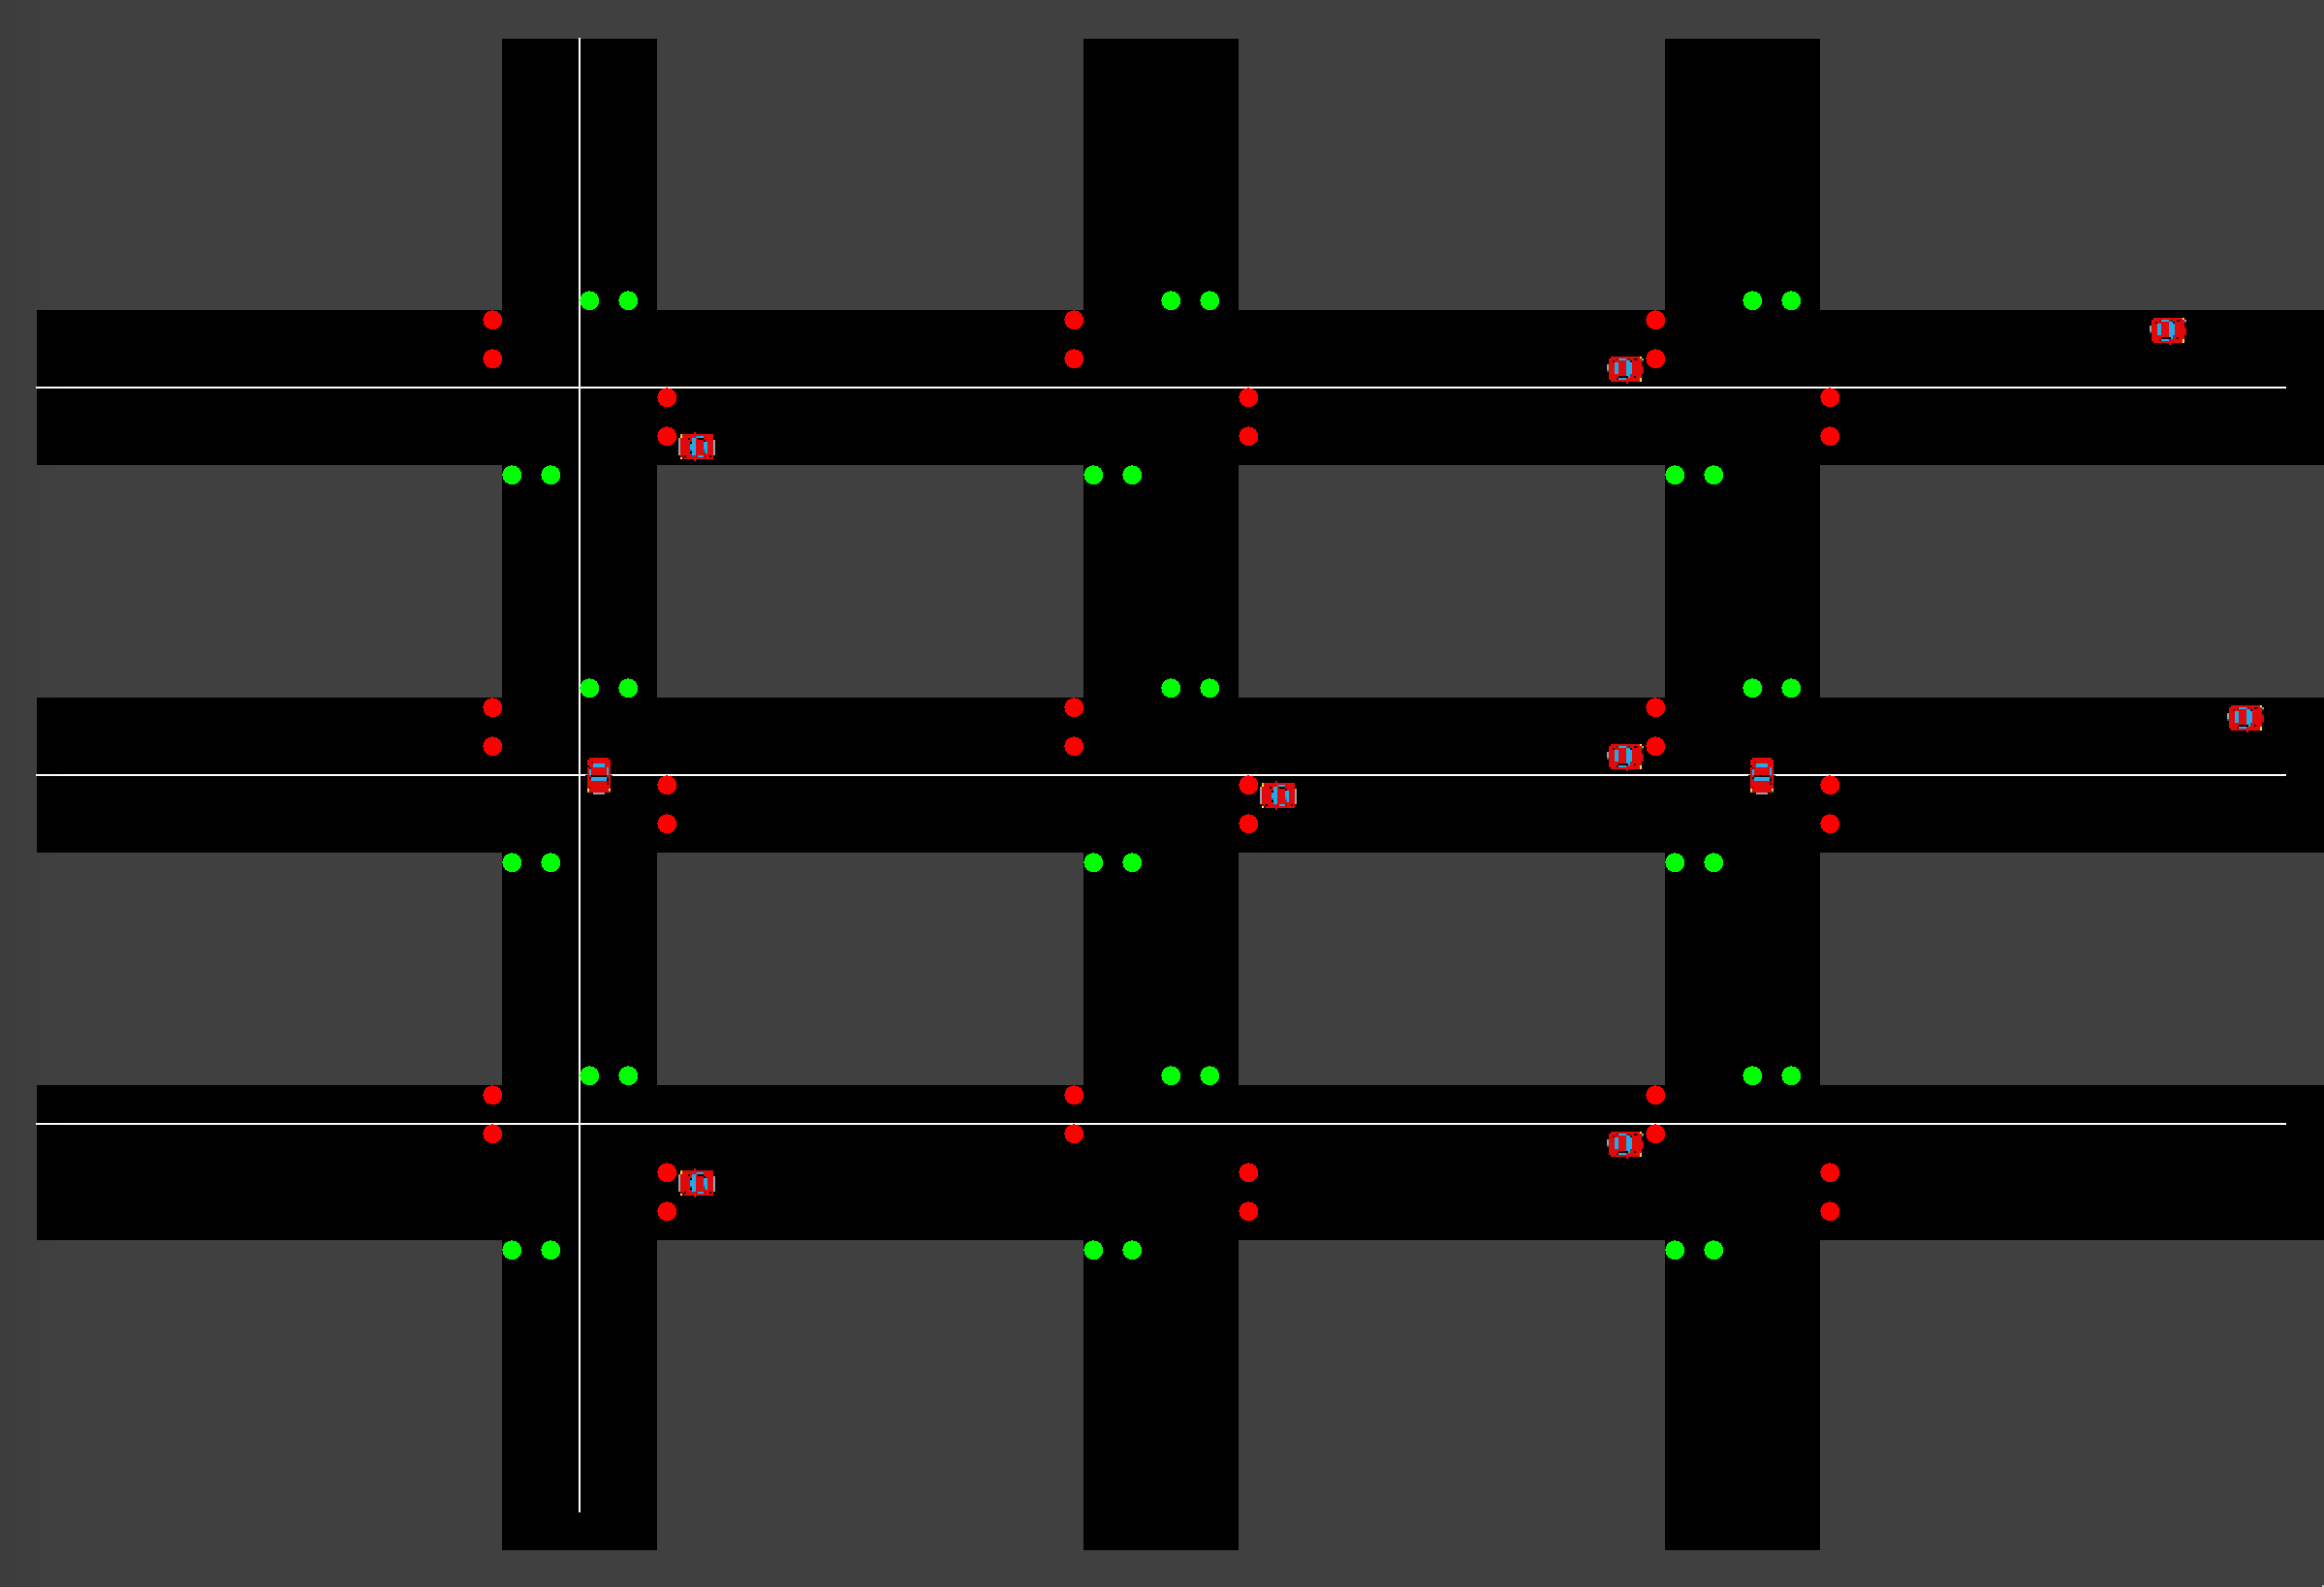
\includegraphics[width=12cm, height=12cm]{pics/trafficSimu}
\centering
\caption{Map bird-eye view}
\end{figure}

\subsection{Aims and objectives}
The over aim of this project is to design traffic simulation engine in order to test the traffic management policy. This project is broken into two section where the first section is the backend structure, which contains the main part of the code as it indicates the functionality of the programme. The second section of the project is the front-end, the main purpose of the Graphical User Interface is to simulate the backend provide user interaction in order to change the parameters. The project has number of objectives to achieve the aims, the following list are the objective to be carried out throughout the project:

\begin{itemize}
\item Research and investigate traffic model and fit it into flexible graphical user interface in order to provide a real life scenario for the user.
\item Setting the aim and the requirements for the implementation.
\item Designing a use-case diagram and class diagram.
\item Design and implement the front-end and the backend of the system.
\item White-box testing the code (should include various testing technique such as unit testing and integration testing techniques).
\item Black-box testing of the system, in order to insure that the requirement are met (this will include functional testing approach).
\item Designing and ind�pendant code.
\end{itemize}



\newpage
\section{Review}

In this section, we will describe various approaches carried out to develop a traffic simulation providing brief context and overview describing various model and classification to design various models. 

 \subsection{Overview}
Traffic simulation modelling is an established tool in order to improve the traffic operation. Over the past six decades, many have contributed in order to develop various traffic simulation models, and many application and experiment has been created in real and synthetic traffic operations. There are various numbers of simulation methods such as dynamic or statistic, macroscopic or microscopic, stochastic or deterministic. Where each models has to be used for a specific application as every model has its own limitation and logic in traffic control system.  In macroscopic model traffic consider the traffic flow on the entire vehicle where in microscopic every vehicle behaves individually depending on its interaction with other vehicles whereas mesoscopic models has combination of both categories. The traffic simulations are classified based on their detail levels and functionalities, in the diagram below various type classification are divided into categorise   as shown in the diagram below.

\begin{figure}[h]
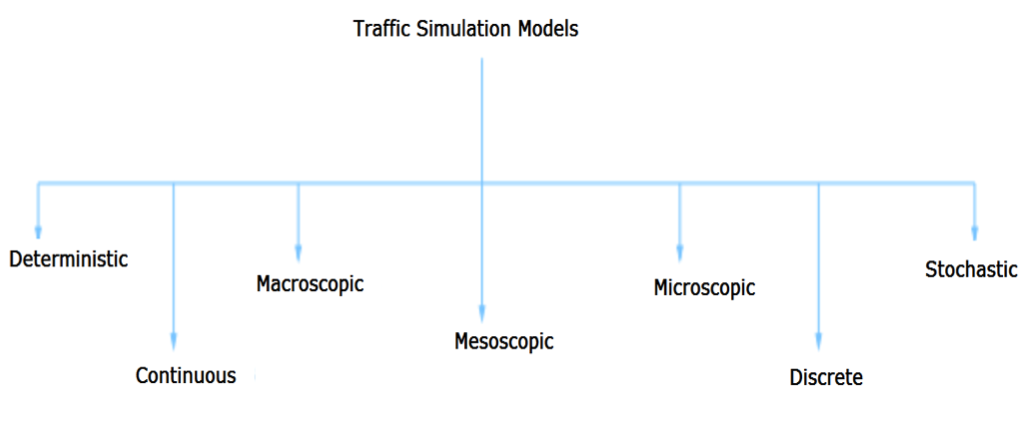
\includegraphics[width=14cm]{pics/simulationModel}
\caption{Traffic simulation model}
\centering

\end{figure}

Initially each model is categorized into discrete and continuous depending on how the elements in the system change states, where discrete model is usually preferred   when the objective is to provide realistic and more detailed description in the system.  Secondly the level of detail should be considered which is categorised in Microscopic, Macroscopic and Mesoscopic models. In macroscopic model the interaction and activities detail description are low level, flow rate details are provided such as speed and density. A macroscopic model provides high level detail in their entity and lower level of details in there interaction and activities, where as in Microscopic both interaction and entity level are both represented in higher level , where lane changing and route planning are some significant example of microscopic model. Thirdly based on the process driven for each model, the simulation model can be either deterministic or stochastic .A deterministic models is represented using mathematical model or a logic where a stochastic model processes using functional probability.  

\subsection{Simulation Models for Traffic Control}
 One of the earliest contribution in traffic simulation design was carried out by the Transport Research Laboratory in mid-1951 in United Kingdom, this model was design for highways considering the intersection.  In 1953 another freeway and interstation simulation model was developed in UCLA in United States \cite{mayad}. since then many research and simulation models has been developed rapidly,  such as, May \cite{mayad2},Van Aerde et at \cite{mayad}, Gibson \cite{mayad}, Sab and Stockfisch \cite{sabra}. The problem of traffic simulation, grab based network , various traffic management policies and control approaches such one way street , reverse street and  bloc.kage are extensively studied and various methods are designed to simulate these environments .
 
 \subsection{Macroscopic Model: NETFO an TRANSYT}
 One of the popular approaches in traffic simulation ``microscopic simulation'', the in this model both the system interaction and their entities are high level detail, Where car following, lane change are significant example. One of the earliest microscopic traffic simulation available was NETSIM, this model was initially implemented in 1971 and integrated with TRAF in mid-1980s which was called TRAF-NETSIM, most of simulation in network streets operation was implementable using this model. TRAF-NETSIM provides a high level of accuracy in traffic simulation and is popular in the field of traffic simulation \cite{sabra}. In order to move the vehicle in this model an interval scanning simulation approach will be used to direct each car each second to car following logic to control the traffic and other  possible condition. The TRAF-NETSIM model is operated using the Mante Carlo Process in order to generate in work traffic simulation condition where the vehicles change location in a random process \cite{rathi2}.
 
 \subsection{Microscopic Model: TRAF NETSIM}
 TRANSYT known as ``TRAffic Network StudY Tool'' is single time period optimisation model which was developed in United Kingdom in a Traffic Research Laboratory also known as TRL. there are current various versions of TRANSYT and this model has been applied in for generating traffic simulation globally. In mid-1980s another version of this model was developed in north America known as TRANSYT-7, which is popular traffic simulation used in US.  This model is a signal controlling of traffic in urban areas, the process searches for any fix time signal appearing in the simulation and reduces the delay of each vehicle, this can be done by co-ordinating adjacent signal, remove the platoons of traffic generated in the simulation. This model consist of process of optimisation and traffic model. There is mathematic collocation used in this system known as ``Performance Index'' (PI)  in traffic simulation network using a specific set of signal timing to tune the timing and constantly adjust the PI measurement \cite{chard},in this model the vehicles are not represent individually and all the measurement are made based on average flow rate rather than individual vehicle consideration.
 
 \subsection{Mesoscopic Model: SATURN and CONTRAM}
 CONTRAM stands for ?Continuous Traffic Assignment Model? is a traffic simulation model that control the flow of traffic in the network of the system. This approach treats the groups of cars as a single entity where cars are considered as packets in the network system, therefore the cars that belong to a certain packet will have the same arrival time, and the minimum cost \cite{smith}. The traffic demand in this model are represented as O-D for a given time interval. Where these O-D are used to measure the number of packed assign to the network in order to evaluate uniform flow rate of packet in to the system.
 
  \subsection{Other Models }
There are various other traffic simulation model developed such as TRARR and TOWPAS which were developed for highways traffic management, In these approaches a signal timing optimization has been processed to determine the phase sequence, cycle length, coordination offsets and green time for coordinated arterials and signal intersection. \newline

  


\newpage
\section{Requirement and Design}

\subsection{Requirements}
Design phase of the software development involves several crucial processes and one of them is identifying requirements. Requirements must be specified in a clear and unambiguous way in order to guide the team towards the final aim. Taking into account that,  it is not always possible to meet all the requirements in the given time,  prioritising them into different levels is very  beneficial for any software development project.  Software requirements are divided into two major groups: functional requirements and non-functional requirements. Simply, functional requirements determine system functionalities (e.g. what system should do), and non-functional requirements specify the constraints that will be on the system\cite{msads}.

\begin{figure}[h]
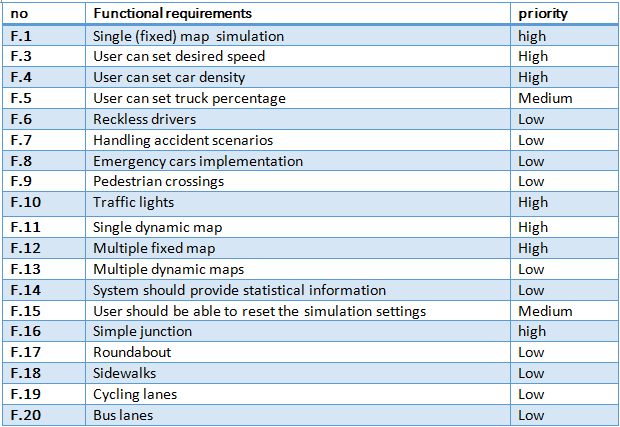
\includegraphics[width=14cm, height=10cm]{pics/FR}
\centering
\caption{Functional Requirements}
\end{figure}

\begin{figure}[H]
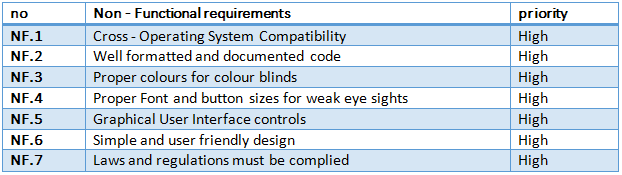
\includegraphics[width=14cm, height=4cm]{pics/NFR}
\centering
\caption{Non-Functional Requirements}
\end{figure}


\subsection{Use Case}

When considering the diagrams to represent system interaction, we see there are variety of them, however not all of them are appropriate for each project. One of the essential diagrams to depict user's interaction with the system is Use Case diagram. Use case diagrams are usually referred to as behaviour diagrams used to describe a set of actions (use cases) that some system or systems (subject) should or can perform in collaboration with one or more external users of the system (actors)\cite{umlucd}.\newline
 
\begin{figure}[H]
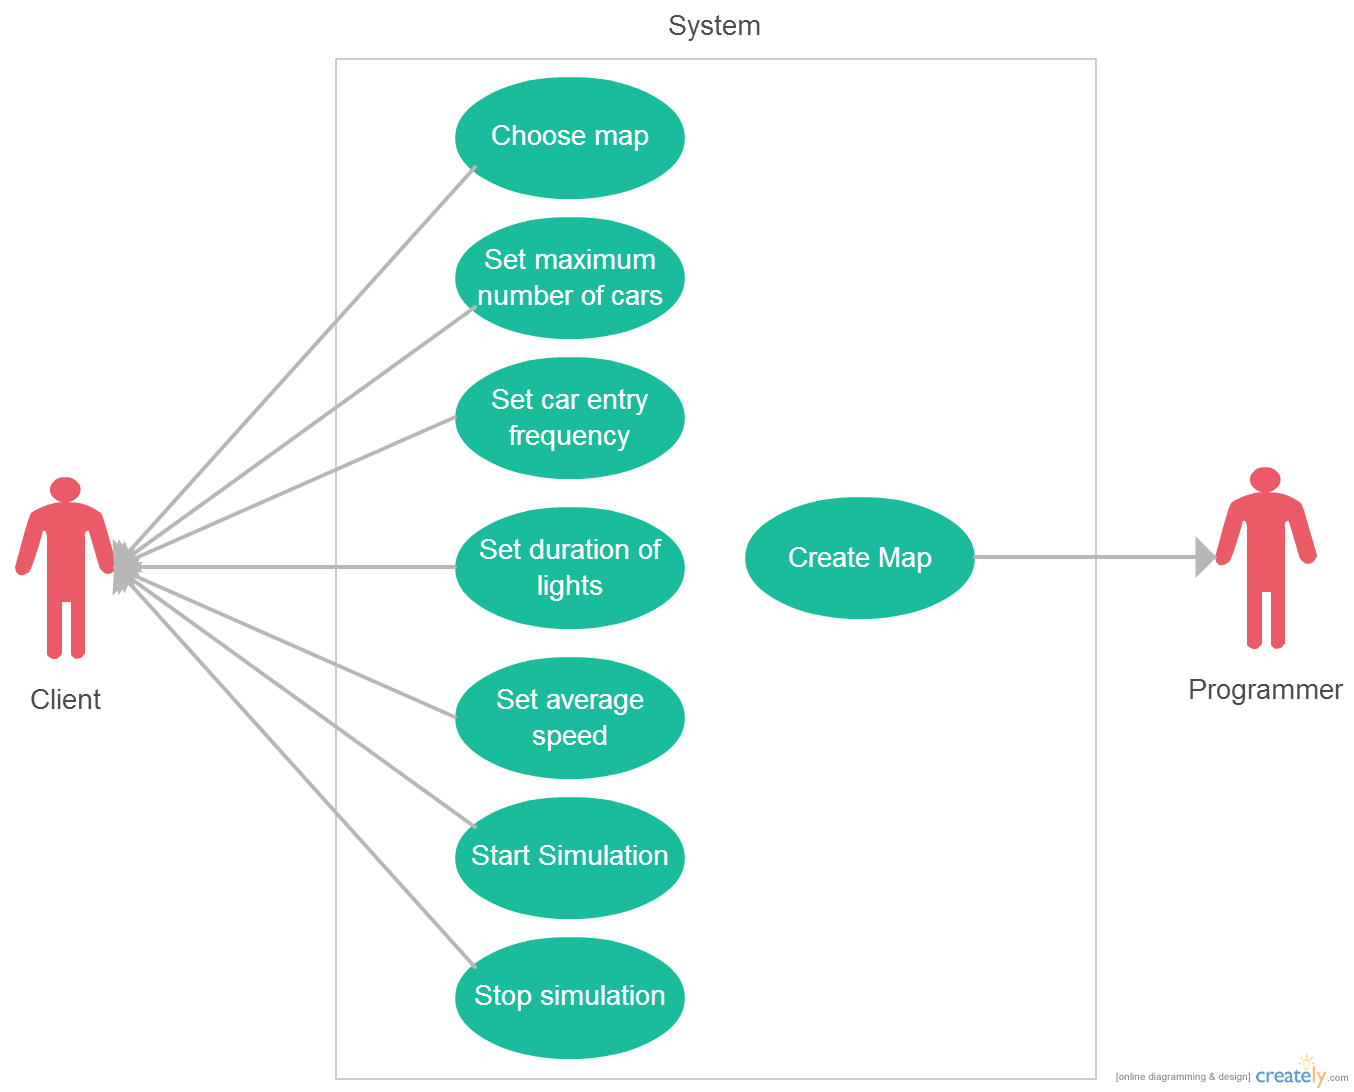
\includegraphics[width=12cm, height=12cm]{pics/useCase}
\centering
\caption{Traffic Simulation Use Case}
\end{figure}

\subsection{Software Development Methodology}
\indent There is a plethora of systems development methodologies, each with differing strengths, weaknesses and target industries. A well-known and traditional methodology used to develop and maintain IT systems is the Systems Development Lifecycle (SDLC) \cite{hoff}. One of the earliest and most established expressions of the SDLC is the waterfall model \cite{Sch95}. The waterfall model can be convenient for certain project because it has been adopted by many and different types of projects and due to some of its advantages. For instance, it recommends a linear approach to software construction, which allows stakeholders to easily understand the processes involved. \newline

\indent However, it also has some issues that need to be taken into consideration when developing IT projects. For example, the project is committed to a frozen set of detailed requirements \cite{larm}, which makes it very difficult to adapt, in case extra requirements are to be added at later stages. What is more, each phase is independent and developed over a fairly long period of time and they cannot be revisited once complete. Large steps are taken in which many decisions are made without the benefit of concrete feedback from realistic implementation and testing \cite{larm}.
 
\subsection{Iterative and Incremental development}
\indent On the other hand, there are other methodologies, such as, the Iterative model, which can be more suitable for certain types of projects. According to Larman, 2005 \cite{larm}, the Iterative development offers support to reduce some problems exacerbated by a linear waterfall model. The Iterative approach consists mainly in developing in short periods of time, providing constant feedback and allowing adaptation \cite{larm}.  This approach has four phases. These are inception, elaboration, construction and transition. Within each phase, there are five disciplines: requirements, analysis, design, implementation (building the software) and test\cite{cadle}. Figure 5 explains how development is none using this models.
 
\begin{figure}[H]
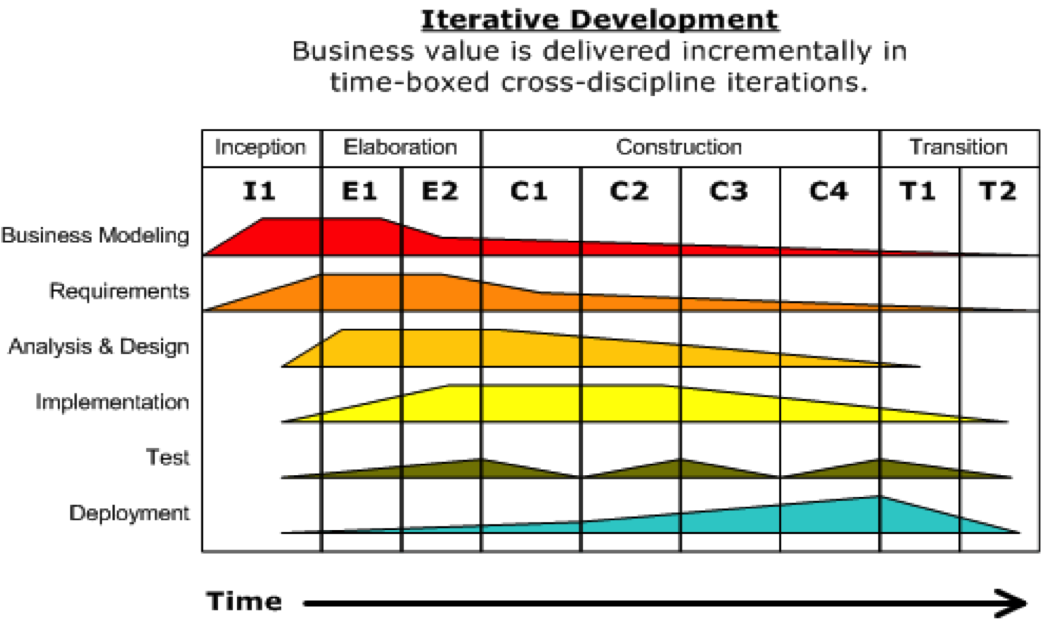
\includegraphics[width=12cm, height=8cm]{pics/methodology}
\centering
\caption{Iterative and Incremental development model}
\end{figure}
 
 In contrast to the waterfall model, in this approach, development is done into a series of short, fixed-length (for example, four week) mini-projects called iterations; the outcome of each is a tested, integrated, and executable system\cite{larm}. These characteristics of this approach were more reflected to our project needs and hence we selected it over the waterfall. We started to develop immediately, after obtaining the system specifications. We decided not to concentrate so much time, in only one particular process, analyzing or designing the system, for example. Instead, we opted to start working on several processes in parallel in order to have some early and visible results of the traffic simulation. \newline
 
\indent Furthermore, we have decided to address the problem in this way, because of the two types of requirements that we aimed to achieve. We defined primary requirements, which were fixed, and secondary requirements, which were evolving over the weeks. Hence, we needed to use a model, such as the Iterative one, that could adapt to our project, and that allowed us to make changes to the requirements, which eventually triggered modifications to the whole system, including the designs, coding and testing. Further advantages\cite{larm} that encouraged us using this approach are summarized bellow:
 
\begin{enumerate}[itemsep=1pt]
\item Risk mitigation: Early rather than late mitigation of high risks (technical, requirements, objectives, usability, and so forth)
\item Agility: Early feedback, user engagement, and adaptation, leading to a refined system that more closely meets the real needs of the stakeholder
\item Managed complexity: The team is not overwhelmed by "analysis paralysis" or very long and complex step
\item Guidance: Early visible progress
\end{enumerate}

%Should this be as a new section or subsection-------------------------
\newpage
%Should this be as a new section or subsection
\section{Back End Design}

\indent The above section described the design for the user interaction for the front end of the software, the following section will cover the design and construction of the simulation. 

\subsection{Constructing the Map}

\indent In the context of the simulation, the game board can be defined as the area in which the siulation is presented. A more precise definition, our game board can be represented as a two dimentional matrix $ G_{i,j} $ where $ i = 1 \dots m $ and $ j = 1 \dots n $. More specifically, 

\begin{figure}[h]
\centering  
\[ 
G_{m,n} = 
\begin{bmatrix}
    g_{1,1} & g_{1,2} & \cdots & g_{1,n} \\
    g_{2,1} & g_{2,2} & \cdots & g_{2,n} \\
    \vdots  & \vdots  & \ddots & \vdots  \\
    g_{m,1} & g_{m,2} & \cdots & g_{m,n} 
  \end{bmatrix} \]
\end{figure}

In this way, the game board gives us a matrix (a grid) which is used as the foundation for identifying the placement of lanes, lights and agents on the board. 

\subsection{Constructing lanes and Junctions}

\indent Using the game board with variable height and width a natural progression was the designing of the lanes. A lane can be thought of as a line which has a starting and end position. The start and end position must reside within the bounds of the two dimensional matrix. Each element of the matrix corresponds to a point on a lane.   
%Single Lane picture 
\begin{figure}[H]
    \centering
    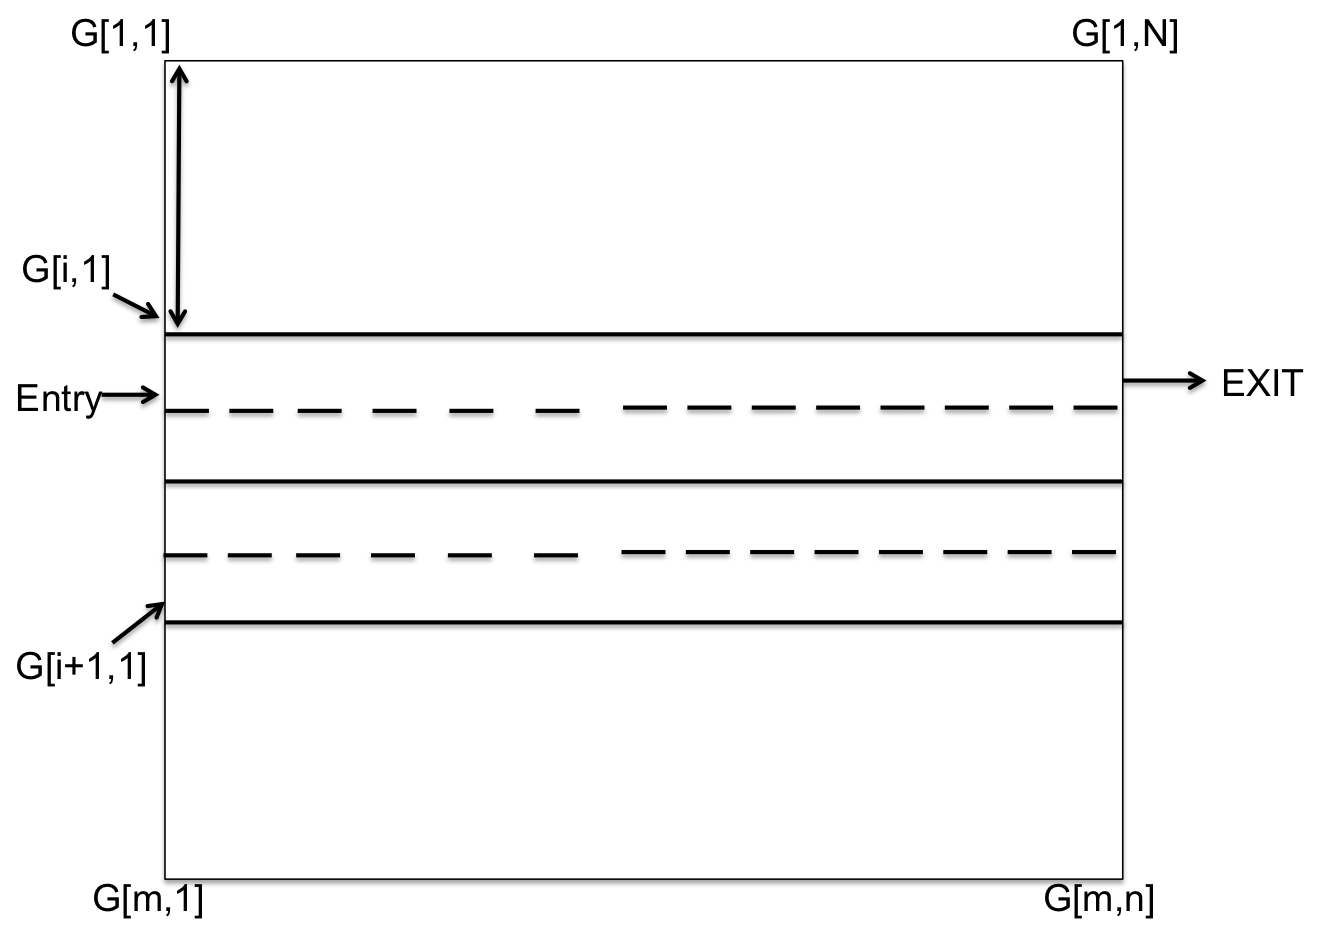
\includegraphics[width=0.8\textwidth]{pics/lane.png}
    \caption{Two lanes on the game board}
    \label{fig:Lanes}
\end{figure}
Figure \ref{fig:Lanes} describes a lane ontop of our game board matrix. \newline
\indent A junction is a crossing of one or more lanes. Each lane has a start and end point. The placement of the junction on our gameboard is as follows. 
%put the junction here 
\begin{figure}[H]
    \centering
    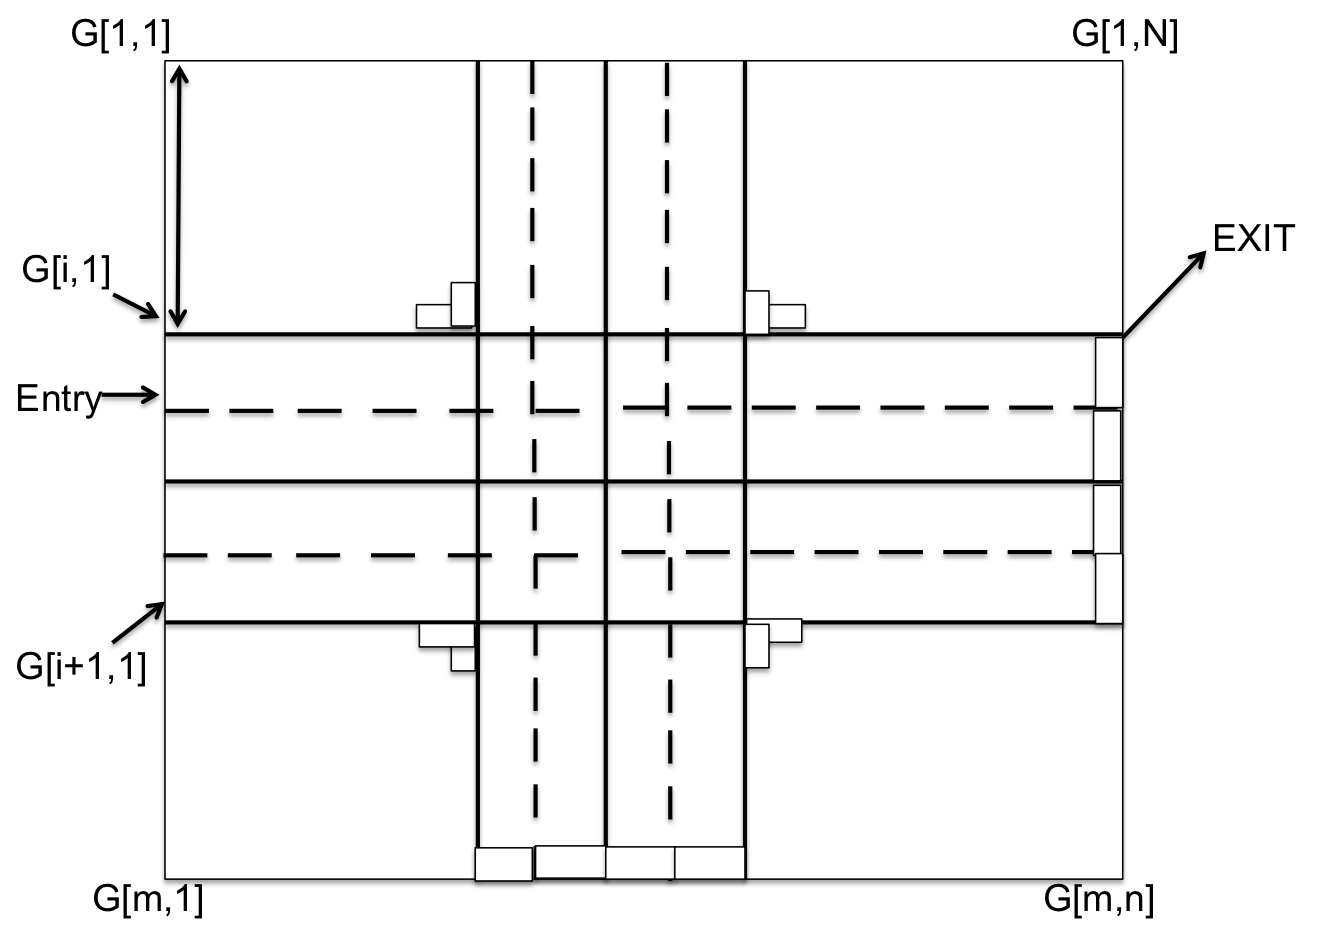
\includegraphics[width=0.8\textwidth]{pics/map.png}
    \caption{Single junction on the Game Board} 
    \label{fig:SingleJunctionPhysical}
\end{figure}
Figure \ref{fig:SingleJunctionPhysical} describes a single junction. The idea of a single junction can be applied to a map with multiple juncitons. Having adressed the construction of the gamebard, lanes and junctions we can move onto the logical components of the lanes and junctions. \newline
\indent Having a designed a physical map we can begin to assign some logical components to it - starting with a single junction consisting of two lanes in the North South East and West directions. Each lane is given an id and direction. The lane id's are odd and even numbers (starting at 1) and the direction of a lane is an integer value ranging from $ 0 \dots 3 $. 
%Logic for map1_1Intersetion
\begin{figure}[H]
    \centering
    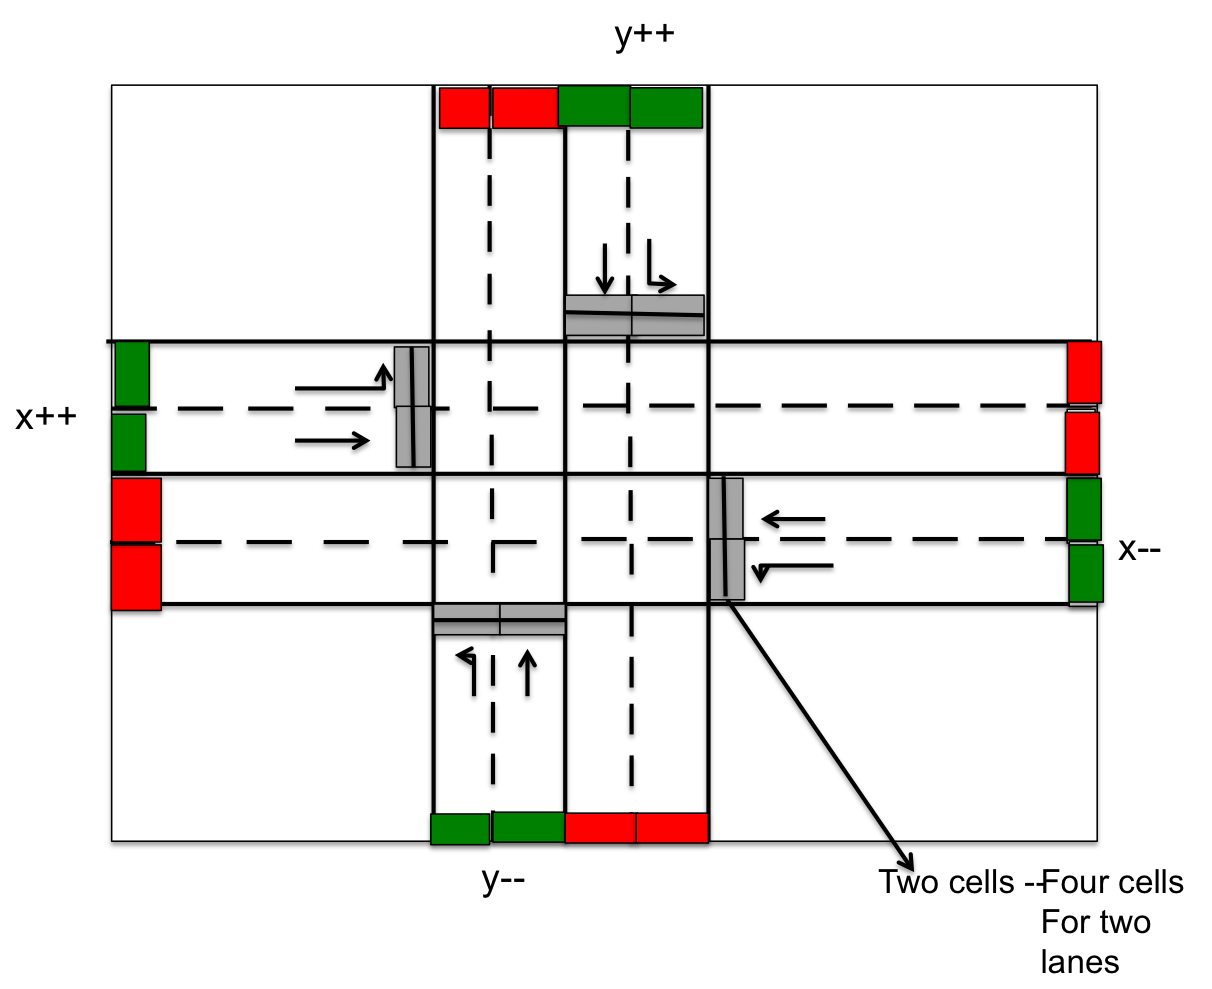
\includegraphics[width=0.8\textwidth]{pics/map2.png}
    \caption{Single junction Logic} 
    \label{fig:SingleJunction}
\end{figure}
In figure \ref{fig:SingleJunction}, a starting cell is given the color green and the end cell red. The lane id and directions are listed to the left of the lanes. The inner most lanes are for vehicles travelling straight hrough a junction and the outer most (odd and even) lanes are for vehicles who will be turning. Using the same logic, this can be applied to a map with the same number of lanes but changing the number of junctions.\newline
%Logic for map2_4Intersetions 
\begin{figure}[H]
    \centering
    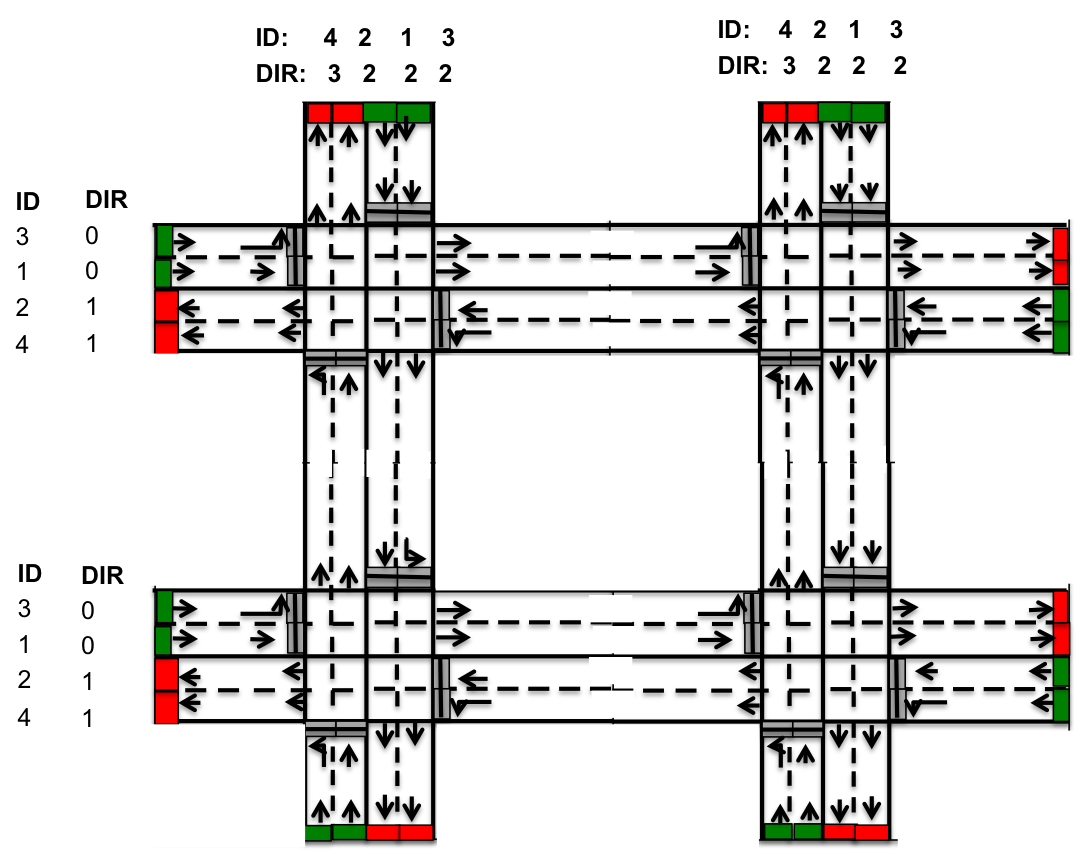
\includegraphics[width=0.8\textwidth]{pics/map3.png}
    \caption{Multijunction lane logic} 
    \label{fig:Multijunction}
\end{figure}

\indent In the same way, a network consisting of multiple lanes and junctions \ref{fig:Multijunction} can be constructed with the same logic used in a grid with a single junction.  


%--------------------------------

\subsection{Class Diagram}
This section explains the class-digram of the entire system. The biggest class is the car class. It has several relations to  other components of the system. However, in the figure bellow, it does not show these links to the respective components, because of page size limitation. Nevertheless, the following explains  briefly, how the Car class is related to the respective classes. 

The class diagram links to the following classes: \texttt{Lane}, \texttt{Cell}, \texttt{Light} and \texttt{Map}.

Finally, the \texttt{GamePanel} class also has an important relation with \texttt{Car} class, as it can have many cars objects. 

\begin{figure}[H]
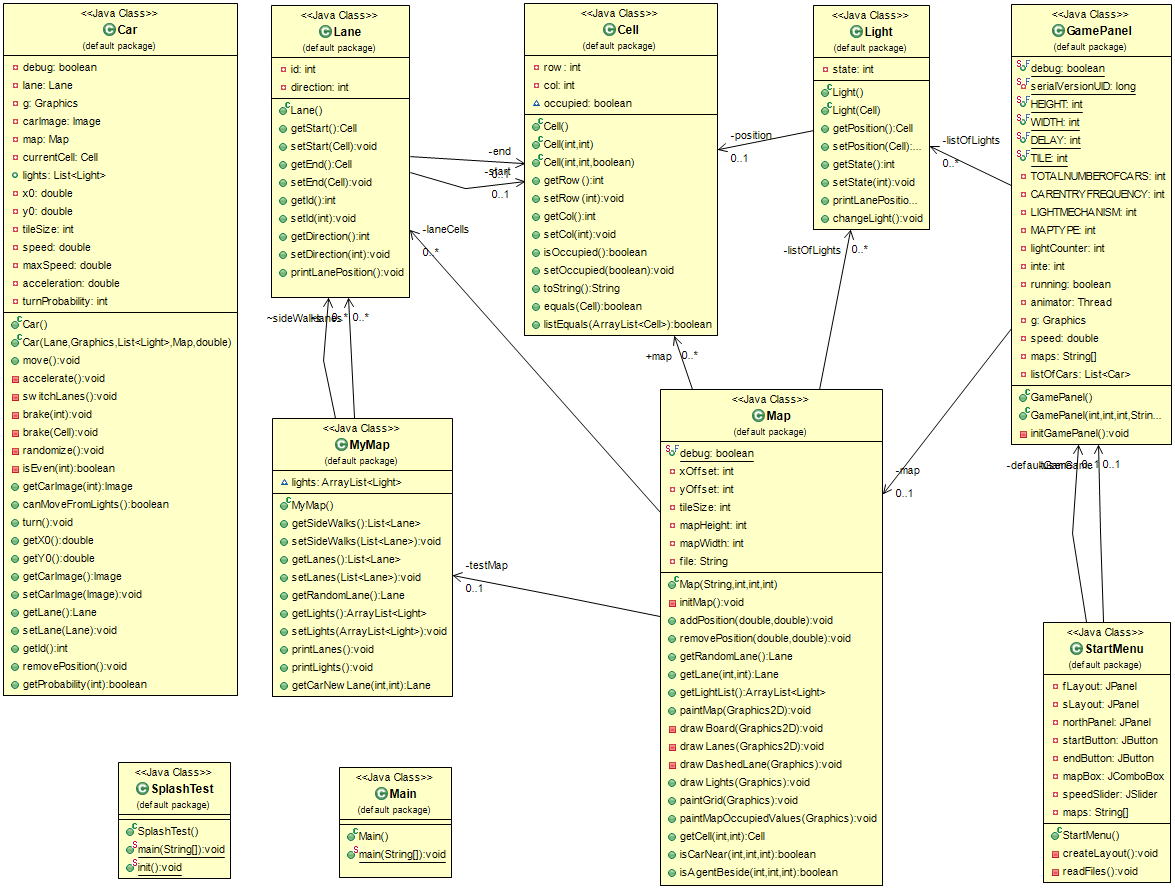
\includegraphics[width=16cm, height=15cm]{pics/classDiagram}
%\centering
\caption{Traffic simulation class diagram}
\end{figure}

 

\newpage
\section{Implementation}
\indent Using the design structure above, our next aim was to create a code which had an independant and portable structure. This section describes how our design translated into code. This section is divided into two subsection; significant implementations and software testing.

\subsection{Significant Implementaion}

\subsubsection{Map and Cell class}
\indent Using the design structure discussed above we proceeded to the next phase - implementation. The implementation rests heavily on the idea of a matrix (used in the \texttt{Map} class) and the design of it's elements. The matrix can be thought of as holding an ordered pair of elements which are objects of the class \texttt{Cell}. A cell is defined by it's \texttt{row}, \texttt{col} and \texttt{isOccupied} boolean value. To read the paramaters to create the map, we used the following external lbraries, 

\begin{enumerate}[itemsep=1pt]
\item jackson-annotations
\item jackson-core
\item jackson-databind 
\end{enumerate}

The class \texttt{Map} holds the an object of class \texttt{MyMap} where the information of the json configuration file is mapped to. The following snippet represents the two lines which were used for the mapping, 

\begin{lstlisting}[language=java]
  ObjectMapper mapper = new ObjectMapper();
  testMap = mapper.readValue(new FileReader(this.file), MyMap.class);
\end{lstlisting}

The bounds of the matrix for $x$ and $y$ were between
\begin{equation*}
 0 \le x \le \texttt{WIDTH} \textnormal{  and  }  0 \le y \le \texttt{HEIGHT}
\end{equation*}
 respectively. The dimentions of the map initially were $0 \leq x \leq 1200$ and $0 \leq y \leq 800$. In order to reduce the amount of computation required by each agent when checking the availability of the next element of the matrix a modification was necessary. A map is created with a hegiht, width and a tilesize. On creation of the map, the tilesize was used to normalize the height and width used to construct the map of cells, 

\begin{equation*}
0 \le x \le \texttt{mapWidth} = \frac{\texttt{WIDTH}}{\texttt{tileSize}}  \textnormal{    and     }  0 \le y \le \texttt{mapHeight} = \frac{\texttt{HEIGHT}}{\texttt{tileSize}}
\end{equation*}

When displaying the grid, it was done with the original dimensions, but resized by the value of \texttt{tileSize}. 
%insert figure matrix here
\begin{figure}[H]
    \centering
    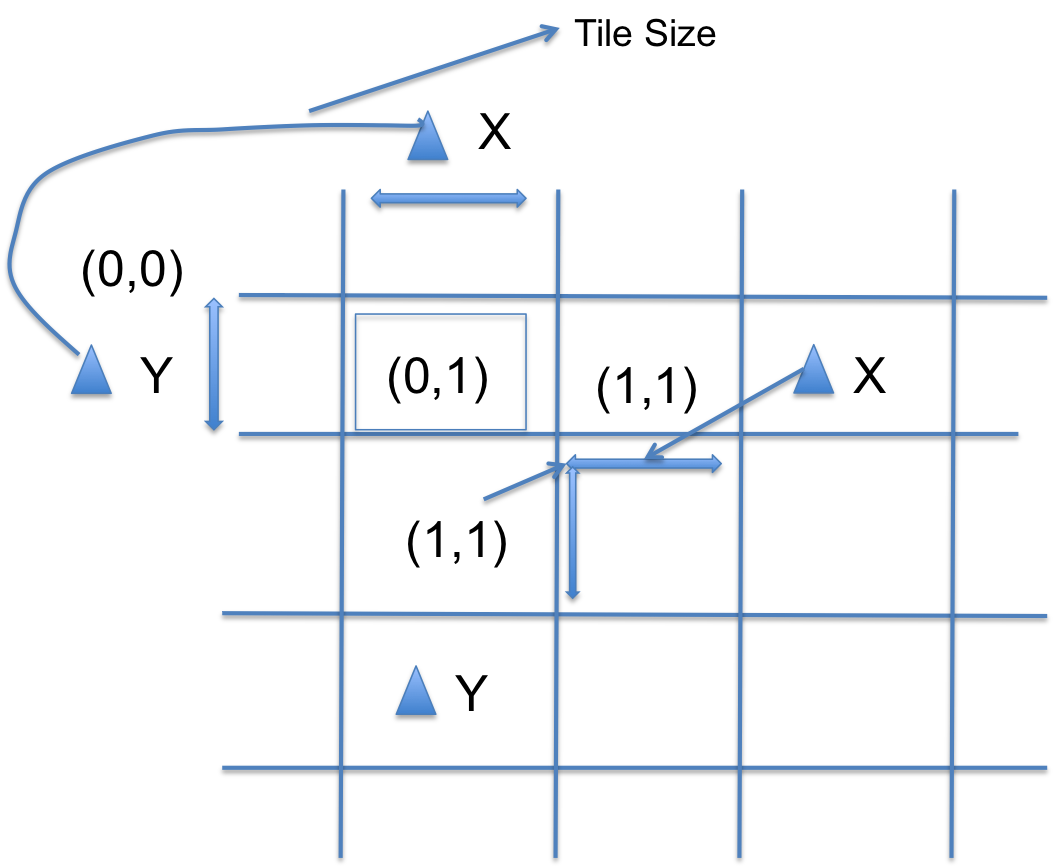
\includegraphics[width=0.8\textwidth]{pics/matrix.png}
    \caption{Expanding the GUI with tileSize}
    \label{fig:tileSize}
\end{figure}
In this way the creation of a map would hold $10^{2}$ less cells than the map which was displayed in the GUI. 

\subsubsection{JSON}
\indent  The json configuration file is used in the class \texttt{Map} the starting and ending positions of lanes, their id's and directions. It also holds the information of the lights and their default values. 

\begin{minipage}[b]{0.45\linewidth}
\centering
\begin{lstlisting}[language=json, firstnumber=1]
  ``lights'': [
    {
      ``state'': 1,
      ``position'': {
        ``row'': 42,
        ``col'': 64,
        ``occupied'': 0
      }
    }
    ...
  ]
\end{lstlisting}
%\caption{Lights in JSON file}
%\label{fig:jsonLights}
\end{minipage}
%%
\hspace{0.5cm}
\begin{minipage}[b]{0.45\linewidth}
\centering
\begin{lstlisting}[language=json, firstnumber=1]
  ``lanes'': [
  {
    ``id'': 3,
    ``direction'': 0,
    ``start'': {
      ``row'': 36,
      ``col'': 2
    },
    ``end'': {
      ``row'': 36,
      ``col'': 118
    }
  }
  ...
]
\end{lstlisting}
%\caption{Lanes in JSON file}
%\label{fig:jsonLanes}
\end{minipage}

\indent The above two code snippets describe the structure of the file. On startup the information in the configuration file would be read in class Map and mapped into the class \texttt{MyMap}. \texttt{MyMap} has methods which can then be accessed when needed by the other classes in the program. Using a json configuration file allowed for information to be easily parsed, and more importantly it allowed to keep all the map information in a single location. The latter point gave rise to a more dynamic code - if a new map was to be accessed a this could be done by using a seperate json file, leaving the rest of the code unmodified. 

\subsubsection{Car Class}


\indent In the method \texttt{move()}, it checks the direction of the car (all cases has the same functionality except how the car is checking if there is a car in front of it). It checks if there is a car in front of it by calling the \texttt{getCell()} of the class \texttt{Map}. If it not occupied it continue by checking if the getter \texttt{canMoveFromLights()} (main details will be found in a latter section). If it returns true it checks if it will turn (main details will be found in a latter section).Then it removes its previous position from the matrix, accelerate to its next position and then update the matrix. 

\indent The method accelerate checks the direction of the car and move it to its next position. It calculates its next position by this logic:

\[ \texttt{direction} = \left\{
  \begin{array}{l l}
    0 & \quad \text{then $x+=$ \texttt{tilesize}\*\texttt{speed} & and $y$ = $y$} \\
    1 & \quad \text{then $x-=$ \texttt{tilesize}\*\texttt{speed} & and $y$ = $y$} \\ 
    2 & \quad \text{then $y+=$ \texttt{tilesize}\*\texttt{speed} & and $x$ = $x$} \\ 
    3 & \quad \text{then $y-=$ \texttt{tilesize}\*\texttt{speed} & and $x$ = $x$} \\ 
    
  \end{array} \right.
\]

\indent Every time cars moves, its calling the boolean getter \texttt{canMoveFromLights()}, which returns if the car can move or not. When it returns that the car cannot move, this means that the car is in front of a light and the colour is red. First thing that this method does is to check the direction of the car. In all cases the method running a for loop of  the list of all the lights. If the positionof the light is the same of the cars (actually 1 point in front of the car) then it checks the colour of the light; if it is green it returns  true if it is red it returns false. The method \texttt{getCarImage()} checks the direction of the car and returns the current picture the car need to have.

\indent For a car to turn there is a condition, to be at a specific point $(x,y)$ in an intersection. This point exists after the every light. For the car to find this point it runs a for loop of all the lights of the map and searches for the current point. The calculation is done as follows, if


\[ \texttt{direction} = \left\{
  \begin{array}{l l}
    0 & \quad \text{and light's $x+1=$ car's $x$ \texttt{and light's $y=$ car's $y$}}\\
    1 & \quad \text{and light's $x-1=$ car's $x$ \texttt{and light's $y=$ car's $y$}}\\
    2 & \quad \text{and light's $y+1=$ car's $y$ \texttt{and light's $x=$ car's $x$}}\\
    3 & \quad \text{and light's $y-1=$ car's $y$ \texttt{and light's $x=$ car's $x$}}\\
    \end{array} \right.
\]


\indent When the car is at that point, then it makes a random decision to turn or go straight. If it makes the decision to turn then it changes its lane by calling the method setLane and passing as parameter a getter \texttt{getLane(laneID, laneDirection)} from the class \texttt{Map}. This getter has two parameters: the lane's id and direction that the car is moving now. This method passes this two variables to the \texttt{MyMap} class method \texttt{getCarNewLane()}. Finally this method calculates the new lane of the car by using this condition:


Let $L(i)$ be the current lane, $i-1$ the previous lane, $i+1$ the next line, $L(i)_{id}$ the id of the lane and $L(i)_{d}$ the direction:


\[ $L_{d}(i-1)$ = \left\{
  \begin{array}{l l}
    3 & \quad \text{and $L_{d}(i-1) = 2$ \texttt{then $L_{id}(i+1) = 3$  and $L_{d}(i+1) = 0$}}\\
    3 & \quad \text{and $L_{d}(i-1) = 0$ \texttt{then $L_{id}(i+1) = 4$  and $L_{d}(i+1) = 3$}}\\
    4 & \quad \text{and $L_{d}(i-1) = 3$ \texttt{then $L_{id}(i+1) = 4$  and $L_{d}(i+1) = 1$}}\\
    4 & \quad \text{and $L_{d}(i-1) = 1$ \texttt{then $L_{id}(i+1) = 3$  and $L_{d}(i+1) = 2$}}\\
    \end{array} \right.
\]


After that the car continues to move in its new direction




%----------------------------------------------------------------------------------------------------------------------------------------------------------------------------------
\subsection{Software Testing}

\indent This section will describe the software testing technique strategy in order to validate and verify the quality of the traffic simulation software; the testing techniques are classified into black-box and white box testing. The black-box and white-box testing will be in every part of the software implementation life cycle.

 \subsubsection{White box testing}
\indent White box testing also known as glass box testing and clear box testing is approach used for debugging of the software where the tester has excellent understanding of the design, structure and the  implementation of the software . In the white-box testing the tester selects random numbers for the input to examine various paths through the program in order determine the required output for the system. One of the advantages of white-box testing is that the tester does not require having a GUI in order to do this testing. There are various methods of white box testing such as unit testing, integration testing and system testing, however the main testing carried out in this project will be unit testing \cite{mauro}.

\subsubsection{Unit testing}
\indent The main testing technique used in the white-box testing in the traffic simulation is the unit testing, where the programmer?s carries out this testing. In the unit testing, component and unit of the code are tested. Where every component or unit of the code contains a small portion of the code, which is usually no longer than the class, a unit usually has few inputs and generates a single output \cite{mauro}.\newline

\textbf{Debugging 1}
\begin{enumerate}
\item {BUGS:} ArrayList bugs
\item Component tested: GamePanel
\item Unit tested: paint()
\item Test case1: for loop
\item Test case2: temporary Arrraylist
\end{enumerate} 

In white-box testing we found a lot of bugs and where they are originated. One of them was that when a car was leaving from the simulation?s map in the car component, it supposed to be removed from the ArrayList of cars. So in every move of the car, it checked if the location of the car was out of the map and, if true it was removed from the list; all that behaviour was placed inside of a loop in the list. But, when the program was running it crashed. However, after an exhaustive analysis of our code, we understood that the bug was created because the ArrayList was inside the loop. Eventually, we found a solution by making a method. This has a temporary empty arraylist that passes all elements of the main arrraylist to the temporary one, so the array does not go out of bound and the system does not crashed anymore. \newline

\textbf{Debugging 2}
\begin{enumerate}
\item {BUGS:} GamePanel
\item Component tested: GamePanel
\item Unit tested: paintMapOccupiedValues()
\item Test case1: If a cell RED $\implies$ cell is occupied %requires some special charaters
\item Test case2: If the cell GREEN $\implies$ the cell is unoccupied
\end{enumerate} 

Furthermore, other critical bug that we encountered was that when we created the matrix and the vision of the car, the agent car supposed stop when the car in front was also stopping. However this did not happened, and therefore caused an error. Consequently the bug there was that the car initialized one matrix for each and every one of the cars. The source of the problem was that each of the cars agents updated its own matrix, thus it was impossible to see if there was any other car in front of it. Nevertheless, we experimented with different solutions and found an effective one, which was to create a universal matrix and pass this matrix to each car.\newline

The paintGrid() method is used to paint the grid cells (which were made in the paint method). So If a cell is painted RED => the cell is occupied, and If the cell is printed GREEN => the cell is unoccupied. This helps us understand if the map is being updated properly. Moreover, it helps us understand if the agents, when moving, are setting their current grid occupied, when they are in it and when they leave - they are setting it as unoccupied. \newline

This method was very helpful to helps us see if the code is working properly and moreover, if the agents are working as they are they were programmed to. It basically, minimizes time spent on debugging - if we did not have it here, and in the event of a bug, we would have to sit through and debug the code for hours, but with this method, it saves a lot of time. \newline


\textbf{Debugging 3}
\begin{enumerate}
\item Component tested: Car
\item Unit tested: Accelerate()
\item Test case1: debug  =  true 
\item Test case2: debug   =  false
\end{enumerate} 

In order to make our white box testing more efficient we have used a preventing debugging approach. In the following case, the certain unit of code is being tested on the car component; car relies vastly on a Boolean value (debug) declared at the top, in order to function in an adequate way. For instance, when the system enters the accelerate method (), and if the value of variable debug is set to true, it will then follow the if (debug) statements, which give critical information, such as id of the lane to the map and hence allows the traffic to move in a respective way. However, if the value is set to false the program will continue without outputting the debugging information to the console.\newline

\textbf{Debugging 4}
\begin{enumerate}
\item Component tested: GamePanel
\item Unit tested: paintGrid(g2d)
\item Test case1: debug  =  true 
\item Test case2: debug   =  false
\end{enumerate} 

This method also helps us with the printing of the grid. A grid indicated the size an agent occupies in the game frame. The grid tells us if the agent moves properly/improperly/ as expected or in some unanticipated way.

 
%--------------------------------------------------
\subsection{Further Software Testing}
\indent This sub section discusses the bugs which where encountred and measures taken to minimize time spent finding them and the aids we used. 
\subsubsection{Debugging tools}
\indent The two debugging methods used were,  

\begin{enumerate}[itemsep=1pt]
\item \texttt{paintGrid()}
\item \texttt{paintMapOccupiedValues}
\end{enumerate}

Both tools were used as debbugging aids. The first method divided the grid into squares with the specified \texttt{WITDH} and \texttt{HEIGHT} of the map. This allowed to see if the proper cell was being occupied as an agent moved through the map. The second method would paint a cell red, if occupied and green if unnocupied giving a visual representation of the location of the agent on the board whether they were moving through the cells and if the correct cells were being occupied. These visual aids helped us significantly in identifying bugs which we were aware of and bugs which were lerking in the shadows and identified with this visual aid. 

%\subsection{Performcance Issues and Solutions}

\subsubsection{Block box testing}
 The black-box testing is one major part of the software implantation testing, it result in reliable functional validity of the system. In this project black-box testing has been done based on the requirement set at the beginning of the project, where any incomplete or any inconsistence behaviour can be simply detected .The black-box testing comes from the perspective of the users and it can take inputs that are either valid or invalid from the user perspective \cite{boris}. \newline
 
The black-box testing is carried out in every phase of project implementation and validation life cycle. In this project all testers were taking part of the black-box testing process, the tester where required to take part in the requirement and analysis phase and produce a plane in the design phase of the project  to meet the requirement throughout the black-box testing \cite{boris}. \newline
 
One of the advantages of the black-box testing is that the tester does not require have any knowledge of the software implementation within the software. In the black-box testing the programmers and the tester work independently. Another advantage of black-box testing is that it exposes any inconsistencies or any ambiguities in the specification requirement \cite{boris}. \newline
 
 \subsubsection{Functional testing }

One of the approaches used in the black-testing is known as the functional testing, where the testing is carried out based on the requirements of the project .In this testing the tester does not require to have a knowledge of the software implantation and the main purpose of functional testing is to acknowledge the user point of view on the finished traffic simulation product \cite{mauro}.


\subsubsection{Trafic simulation blackbox testing}

Due to the fact that this program has few controllers, a bug was found during the phase of the black box testing. The start button was pressed and the simulation was running after a different map is selected and the start button is pressed again both of them are running. The solution to this bug was to check if the GamePanel object is null before start running the simulation. If it was not null it removed the previous one from the Frame.











\newpage
\section{Teamwork}

 \subsection{Group meetings}
 
 In order to work together as a group we have used several well-known processes and tools.\newline
 
We have had group meetings, normally once a week but some times meetings twice a week were necessarily. This happened during the first stages of the project when we were planning the work and formalizing the requirements. The first meetings were fairly long, as there were numerous ideas and contributions by all team members. However, these meetings were successful as most of the times we managed to agreed on each other?s views and hence produced realistic short-term plans and task. \newline
 
The meetings were informal, but there was always an agenda to be followed. A team member was always responsible for taking the minutes of the meetings and uploading them on the online group work repository, such as Dropbox. The agendas created were crucial to guide the meetings and the project. The priority of these, discussed the progress of the team and well as individual work done by members. Based on the work and reports delivered, we proceeded to address problems arising and give attention to areas where more work was required. We concluded the meetings planning on tasks for the following week and points to be discussed for next time, including time and date.

 \subsection{Requirements and Design processes}
 The Requirements and Design processes were completed fairly successful, since we worked and communicate frequently and also provided feedback, which was further improved.\newline
 
During the first stages of the system lifecycle, the requirements were vague and hence there were different interpretations by team members. Nonetheless, we analyzed the systems specifications and different traffic management policies and reached an agreement to produce two types requirements, as explained in section two. Consequently, we decided to go ahead developing with the primary requirements. Though, we also took into consideration that we could have to adjust the requirements and design, according to progress of implementation process and the whole project itself. \newline
 
For this process we worked the five of us together, sometimes the worked was produced in the computer laboratories or in the library, where we booked the study group rooms. We have used various types of tools and technologies, such as UML, Microsoft Project to produce diagrams and charts. Much simpler techniques, such as pen and paper were used to produce uses-cases and to model the classes, objects and the entire systems. In several occasions, we were required to do individual research and produce requirements based on it and share the work on Dropbox.

\subsection{Implementation and testing} 
For these process the work was produced slightly different. Since work was divided into small groups, each team had its own way to approach respective task. \newline

The team of programmers has been implementing the requirements, as a team of two people by meeting up several times a week. They have also been producing worked individually at their own time. Most of the worked was completed at the KCL labs facilities as well as using members own computers and properties. In order to communicate outside university hours, the two members have used social media channels, such as Skype and whatsapp. The programmers have coordinated fairly well, as they have used GitHub, in a professional manner to share their code and to make any changes as needed. \newline

Similarly, the team of Testers has been also meeting in the library at group study rooms. Sections of half a day have been spent and a substantive effort was put on testing the different components of the system. In addition, testers were required to do some preparation individually by studying certain parts of the code, before meeting up, so progress could be made during the testing meetings. During the Testing sessions, specific test cases were tested for finding the bugs on certain functions and classes. The group also used Skype and whatsapp for communication purposes and to organize the work. 

\subsection{Documentation and main tools for collaboration} 

For the documentation process, work has been produced individually, however, everyone has contributed equally and also helped each other by providing useful feedback. Certain parts of this final report were produced according to members' responsibilities with the project. For example, programmers have written the implementation part, as they have full understanding of the code and analysts have conducted the literature review because this task was fairly independent from other processes of the project or system. In addition, short meetings were scheduled once a week to discuss the progress of the final report and documentation. Short-term deadlines were set for this process, in order to encourage everyone to produce a good quality work and not leave the majority of work for the last minute.\newline

Upon completion of the tasks, members uploaded the work on Dropbox to the group's repository and one person was in charge of putting all the parts together, and formatting the report using Latex mark-up language.\newline  

For this process, the communications channels mention above have been used significantly to coordinate with the different groups as well as all team members. The following  explains the main tools utilised to complete the project: 

\begin{enumerate}
\item GitHub
\begin{enumerate}
\item Have been used to share the source code and update the progression of the software implementation.

\end{enumerate} 
\item Dropbox
\begin{enumerate}
\item Have been used to record meeting minutes, share references and documentation, update each member of group of each meeting in cases where they miss the meeting.

\end{enumerate} 
\item Skype 
\begin{enumerate}
\item Have been used for conference calls, and in order to consume time for meeting arrangements.

\end{enumerate} 
\item Whatsapp 
\begin{enumerate}
\item Have been used to inform the group when we had meetings and for instant chatting and updates.

\end{enumerate} 
\item Latex 
\begin{enumerate}
\item Have been used to put all the work and documentation together and formatting the report in a well presentable way. 
 
\end{enumerate} 
\end{enumerate}
  
  


\newpage
\section{Evaluation}
This section will focus on critically evaluating the overall project and the performance of the team, outlining strengths and weaknesses of the group work, discussion of whether all the requirements met and as well as learning outcomes and future work. 

\subsection{Teamwork Evaluation}

Achieving a good and productive teamwork is the goal of many organizations nowadays. When looking at the successful projects, it is evident that there is a strong teamwork behind it. However, achieving such a teamwork is not always straightforward. In order to be able to evaluate our work critically, it is crucial to understand characteristics of an effective teamwork in the first place. "The most effective teamwork happens when individual contributors harmonize their efforts and work toward a common goal"\cite{wmtwe}. According to Demand Media, the main characteristics of an effective team work are as following:

\begin{itemize}
\item Good leadership
\item Adaptability
\item Diversity
\item Effective Communication
\item Skilled Conflict Management ( Demand Media, 2015)
\end{itemize} 

Although the overall performance of our group was satisfying, the team lacked some of the qualities of a good teamwork. When evaluating the qualities of our team, we noticed that we had all the 5 characteristics with some minor issues. Lacking a good time management and control system originated several problems such as delays in producing tasks on time. However, having a good communication and conflict solving mechanism helped to overcome those obstacles. One of the vital aspects to be successful is to fully understand strengths and weaknesses of the team.  To have a better view on evaluation of the work throughout the project, we produced full list of our strengths and weaknesses:\newline

\textbf{Strengths}
\begin{itemize}
\item Effective communication - Having a good communication amongst team members was one of the aspects that helped to boost our performance. Every team member was easily reachable through variety of channels including Whatsapp, Skype and Facebook. 
\item Enthusiasm -  Every team member had been very enthusiastic about the project, which in its turn helped everyone to work towards the common goal.
\item Adaptability - This helped the team to overcome obstacles that were caused by choosing inappropriate development model in the beginning of the project and enabled us to quickly adapt more appropriate model.
\item Effective Conflict Solving mechanism - Conflicts in a team work are inevitable and our project wasn't and exception. One of the main conflicts arose between 2 programmers when they had different approach and view on implementation. However a good communication and conflict solving skills help to resolve it swiftly.
\item Diversity - Having team members skilled and experienced in different areas has played a key role to develop each field of the project in parallel.
\end{itemize}  


\textbf{Weaknesses:}
\begin{itemize}
\item Time management -  Having a poor time management have caused delays in producing tasks on time and falling behind the work plan towards the end of project. Although team managed to meet the requirements by working harder towards the end of the project, time management is one area that needs improvement.
\item Role allocation fault - Designating testing role to non-programmers was a naive mistake that was made during the initial stages. This put members with less programming experience in a desperate situation and caused delays in progression of the implementation. Involvement of programmers in this task resolved the problem.
\item Poor meeting management -  One of the weak sides of the team was long and less productive meetings. Having a proper and precise agendas for each meeting could have achieved shorter and better meetings.
\item Stubbornness - Stubbornness is an issue that many team project's suffer, causing diversion from working towards the common goal. This issue, however, had been ruled out half way through the project which boosted the performance in the later stages of the development.
\end{itemize}  

\subsection{Requirements evaluation}
  The purpose of the requirements evaluation is to check whether the team has achieved its goals set in the initial stage. Evaluation proved that project have successfully managed to meet the high priority requirements. Implementation of the lower priority requirements were subject to available time. Hence, they remain unachieved due to strict time constraint. Nevertheless, those requirements will be implemented in the future and are part of the future work plan. Scalable design of the software will allow developers to add even more advanced features to the simulation. Tables below highlight all the functional and non-functional requirements that have been implemented.

\begin{figure}[H]
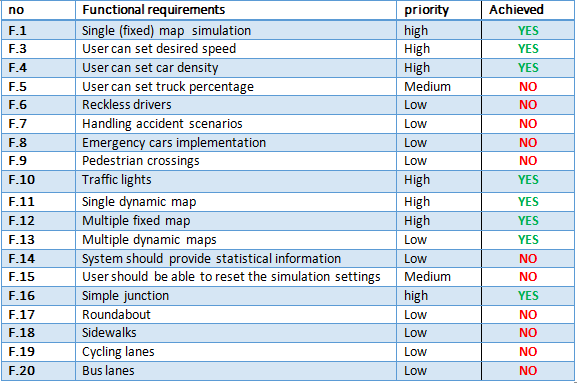
\includegraphics[width=14cm, height=10cm]{pics/FR_EVAL}
\centering
\caption{Functional Requirements evaluation}
\end{figure}


\begin{figure}[H]
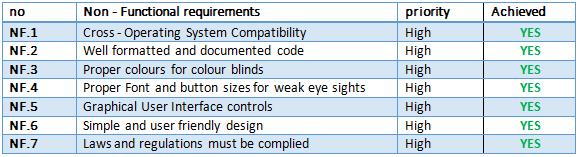
\includegraphics[width=14cm, height=4cm]{pics/NFR_EVAL}
\centering
\caption{Non-Functional Requirements evaluation}
\end{figure}

\subsection{Learning Outcomes}
Getting involved in this project has been very beneficial to every team member in different ways. First of all, the project resembled the real life workplace environment, thus it was very valuable experience and preparation for the future life. Besides that, team members also improved their technical and non-technical skills. One of the most important learning outcomes of the project was understanding the importance of the team work. It gave us the idea of an effective team and how it can be achieved.




\newpage
\section{Code}

\begin{lstlisting}[language=java]
/*Authors : Iordanis Paschalidis, Anthony Tsiopoulos
 * 
 * Class   : This is the main file - the entry point of the program
 */
public class Main {
   
  public static void main (String [] args) throws InterruptedException{
    StartMenu gui = new StartMenu(); 
    gui.setSize(1200,920);
    gui.setVisible(true);
    
    }

}
\end{lstlisting}

\newpage 

\begin{lstlisting}[language=java]
/*Authors : Iordanis Paschalidis, 
* Anthony Tsiopoulos 
* 
 * 
 * Class  : GamePanel.
 * This class is responsible for building the GamePanel. A GamePanel is the immediate
 * class in the hierarchical view of the class diagram. The class is responsible for the 
 * overall control of the game. 
 * 
 * Moded  : 03/06/15
 * 
 */

import java.awt.*;
import java.awt.image.BufferedImage;
import java.io.IOException;
import java.util.ArrayList;
import java.util.Iterator;
import java.util.List;
import java.util.Random;
import java.util.concurrent.ConcurrentHashMap;
import java.util.logging.Level;
import java.util.logging.Logger;

import javax.swing.JPanel;

import com.sun.xml.internal.ws.policy.privateutil.PolicyUtils.Collections;

public class GamePanel extends JPanel implements Runnable {

  public static final boolean debug = false;
  private static final long serialVersionUID = 1L;
  public static final int HEIGHT = 800; // 600
  public static final int WIDTH = 1200; // 800
  public static final int DELAY = 15;
  public static final int TILE = 10;
  private int TOTALNUMBEROFCARS;
  private int CARENTRYFREQUENCY;
  private int LIGHTMECHANISM; 
  private int MAPTYPE;
  private int lightCounter = 0;
  private int inte = 0;
  private boolean running = true;
  private Thread animator;
  private Graphics g;
  private Map map;
  private double speed; 
  private String maps[];
  private List<Car> listOfCars;
  private List<Light> listOfLights; 
  
  
   

  /**
  * This is the default constructor for the game 
  */
  public GamePanel() {
    setDoubleBuffered(true);
    
    this.TOTALNUMBEROFCARS = 100; 
    this.CARENTRYFREQUENCY = 10; // in miliseconds 
    this.LIGHTMECHANISM = 350; 
    this.MAPTYPE = 1; 
    initGamePanel();
    
  }
  
  /**
  * This constructor sets the user specified values at the start screen
  *  
  * @param TOTALNUMBEROFCARS
  * @param CARENTRYFREQUENCY
  * @param LIGHTMECHANISM
  * @param MAPTYPE
  */
  public GamePanel(int TOTALNUMBEROFCARS,int CARENTRYFREQUENCY, int LIGHTMECHANISM, String []maps,int MAPTYPE,double speed) {
    setDoubleBuffered(true);
    this.TOTALNUMBEROFCARS = TOTALNUMBEROFCARS; 
    this.CARENTRYFREQUENCY = CARENTRYFREQUENCY; 
    this.LIGHTMECHANISM = LIGHTMECHANISM; 
    this.maps = maps; 
    this.MAPTYPE = MAPTYPE; 
    //this.speed = speed; 
    initGamePanel();
  }
  
  
  
  /**
  * Private method which sets the map type
  */
  private void initGamePanel() {
    try {
      map = new Map(``res/''+maps[MAPTYPE], WIDTH, HEIGHT,
      TILE);
    } catch (IOException e) {
      e.printStackTrace();
    }
  }
  
  @Override
  public Dimension getPreferredSize() {
    return new Dimension(WIDTH, HEIGHT);
  }
  
  @Override
  public void addNotify() {
    super.addNotify();
    animator = new Thread(this);
    animator.start();
  }
  
  @Override
  public void paint(Graphics g) {
    super.paint(g);
    Graphics2D g2d = (Graphics2D) g;
    
    // Draw map
    map.paintMap(g2d);
    map.drawLights(g2d);
    
    // Draw the images for the cars
    for (Car car : listOfCars) {
      g2d.drawImage(car.getCarImage(), (int) car.getX0() * TILE,
      (int) car.getY0() * TILE, this);
    }
    
    // For testing purpose
    if (debug) {
      map.paintGrid(g2d);
      map.paintMapOccupiedValues(g2d);
    }
    g.dispose();
  }
  
  @Override
  public void run() {
    
    // Create the list of cars
    //This solves the repaint bug - array list was previously unlocked, now locked and unlocked and given to thread 
    listOfCars = java.util.Collections.synchronizedList(new ArrayList<Car>()); 
    listOfLights = java.util.Collections.synchronizedList(new ArrayList<Light>());  
    
    
    while (running) {
      clearOutMApCar();
      listOfLights = map.getLightList();
      
      if( lightCounter % LIGHTMECHANISM == 0 ){
      this.lightMechanism();
    }
    lightCounter++; 
    
    try {
      if ((inte % CARENTRYFREQUENCY == 0)) {
      if (listOfCars.size() < TOTALNUMBEROFCARS) {
        Lane lane = new Lane();
        lane = map.getRandomLane();
        Car car = new Car(lane, g, listOfLights, map,speed);
        listOfCars.add(car);
      }
    }
    for (Car car : this.listOfCars) {
      car.move();
    }
    inte++;
    Thread.sleep(DELAY);
    repaint();
  } catch (InterruptedException ex) {
    Logger.getLogger(GamePanel.class.getName()).log(Level.SEVERE,null, ex);
  }
}
}
  
  
  /**
  * This method removes the cars from the map when they 
  * have passed the maps boundaries. 
  */
  public void clearOutMApCar() {
    List<Car> listOfCars2 = listOfCars;
    Iterator<Car> i = listOfCars2.iterator();
    while (i.hasNext()) {
      Car s = i.next(); // must be called before you can call i.remove()
      if (shouldRemoveFromTheList(s)) {
        s.removePosition();
        i.remove();
      }
    }
  }
  
  
  /**
  * This method checks the direction of the car and compares 
  * it to the bounds of the map. If the cars next value exceeds 
  * the bounds, then the car should be removed from the map. 
  * 
  * @param c
  * @return boolean
  */
  private boolean shouldRemoveFromTheList(Car c) {
    
    if (c.getLane().getDirection() == 0) {
      if (c.getX0() > c.getLane().getEnd().getCol()) {
        return true;
      }
    } else if (c.getLane().getDirection() == 1) {
      if (c.getX0() < c.getLane().getEnd().getCol()) {
        return true;
      }
    } else if (c.getLane().getDirection() == 2) {
      if (c.getY0() > c.getLane().getEnd().getRow()) {
        return true;
      }
    } else {
      if (c.getY0() < c.getLane().getEnd().getRow()) {
        return true;
      }
    }
    return false;
  }
  
  /**
  * This method is used for debugging, just to print the lights location
  * which are read from the JSON file 
  */
  private void printL(){
    for(Light l:listOfLights){
    }
  }
  
  
  /**
  * This method takes each light in the the list of lights and changes 
  * their values depending on their default state 
  */
  private void lightMechanism(){
    for(Light l:listOfLights){
      l.changeLight();
    }
  }
  
  
  }
    
\end{lstlisting}
\newpage

\begin{lstlisting}[language=java]
/*Authors : Iordanis Paschalidis, 
* Anthony Tsiopoulos 
 * 
 * Class  : Car
 * This class is responsible for creating a car.
 * The class implements runnable, so the run() method is
 *is provided as method in the class. An object of the 
 *class Car is a Runnable object.   
 * 
 * Moded:  03/06/15
 * 
 */

import java.awt.*;
import java.util.ArrayList;
import java.util.List;
import java.util.Random;
import java.util.logging.Level;
import java.util.logging.Logger;

import javax.swing.ImageIcon;
import javax.swing.JPanel;
import javax.swing.plaf.synth.SynthSeparatorUI;

public class Car {

  private boolean debug = false;
  private Lane lane;
  private Graphics g;
  private Image carImage;
  private Map map;
  private Cell currentCell;
  public List<Light> lights;
  private double x0;
  private double y0;
  private int tileSize = 10;
  private double speed; // = 0.01;
  private double maxSpeed = 0.03;
  private double acceleration = 0.001;
  private int turnProbability = 4; 

  public Car() {
    Image im1 = getCarImage(lane.getDirection());
    }

  public Car(Lane lane, Graphics g, List<Light> lights, Map map, double speed) {

    Image im = getCarImage(lane.getDirection());
    this.lane = lane;
    this.g = g;
    this.setLane(lane);
    this.currentCell = lane.getStart();
    this.x0 = currentCell.getCol(); // initial position
    this.y0 = currentCell.getRow(); // initial position
    this.lights = lights;
    this.map = map;
    this.speed = speed; 

    }

  /**
   * This method is responsible for moving a car. It checks the if the cell in
   * front of it is occupied and it proceeds to accelerate, otherwise it will
   * brake.
   * 
   * @throws InterruptedException
   */
   public void move() throws InterruptedException {
     
     switch (lane.getDirection()) {
       case 0:
       
       if (!map.getCell((int) x0 + 2, (int) y0).isOccupied()) {
         
         if (this.canMoveFromLights()) {
           
           if(getProbability(turnProbability)){
             turn();
           }
           this.removePosition();
           accelerate();
           map.addPosition(x0, y0);
           
           //}else if(!map.getCell((int) x0 + 2, (int) y0).isOccupied() && map.isAgentBeside((int)x0, (int) y0,getLane().getDirection())){ 
           //  
           //  switchLanes();
           //  this.removePosition();
           //  accelerate();
           //  map.addPosition(x0, y0);
           // 
         }
       }
       break;
       
       case 1:
       
       if (!map.getCell((int) x0 - 2, (int) y0).isOccupied()) {
         
         if (this.canMoveFromLights()) {
           
           if(getProbability(turnProbability)){
             turn();
           }
           this.removePosition();
           accelerate();
           map.addPosition(x0, y0);
         }
       }
       break;
       
       case 2: //y++
       if (!map.getCell((int) x0, (int) y0 + 2).isOccupied()) {
         
         if (this.canMoveFromLights()) {
           
           if(getProbability(turnProbability)){
             turn();
           }
           this.removePosition();
           accelerate();
           map.addPosition(x0, y0);
           
         }
       }
       break;
       case 3:
       
       if (!map.getCell((int) x0 , (int) y0 - 2).isOccupied()) {
         
         if (this.canMoveFromLights()) {
           
           if(getProbability(turnProbability)){
             turn();
           }
           this.removePosition();
           accelerate();
           map.addPosition(x0, y0);
           
         }
       }
       break;
     }
   }
   
   /**
   * This method moves the car in a direction. The directions is decided by
   * first checking the id of the lane. For an even id, the car is travelling
   * in a northbound or westbound lane. if the id is odd: The car is in a lane
   * travelling in a southboun/eastbound direction.
   * 
   * @throws InterruptedException
   * 
   */
   private void accelerate() throws InterruptedException {
     //System.out.println(x0 +''           ``+y0);
     // Increase speed by dx/dy (acceleration) in either direction
     if (speed < maxSpeed) {
       speed += acceleration;
     }
     
     if (debug) {
       System.out.println(``Lane id: `` + getId());
     }
     
     
     if (isEven(this.getLane().getId())) {
       if (lane.getDirection() == 3) {
         y0 -= tileSize * speed;
         if (debug) {
           System.out.println(``In y0--'');
           System.out.println(``Dir: 3 ``);
         }
       } else if (lane.getDirection() == 1) {
         
         x0 -= tileSize * speed;
         if (debug) {
           System.out.println(``In x0--'');
           System.out.println(``Dir:  1'');
         }
       }
     } else { // ODD
       
       if (lane.getDirection() == 0) {
         
         x0 += tileSize * speed;
         if (debug) {
           System.out.println(``In x0++'');
           System.out.println(``Dir: 0 ``);
         }
       } else if (lane.getDirection() == 2) {
         
         y0 += tileSize * speed;
         
         if (debug) {
           System.out.println(``In y0++'');
           System.out.println(``Dir: 2 ``);
         }
       }
     }
   }
   
   /**
   * This method is for a vehicle to switch from their current lane to the
   * lane next to them
   * 
   * @throws InterruptedException
   */
   @SuppressWarnings(``unused'')
   private void switchLanes() throws InterruptedException {
     
     if (isEven(lane.getId())) {
       
     } else { // ODD
       
       if (currentCell.getRow() == lane.getStart().getRow() && lane.getDirection() == 0) {
         y0 += tileSize * speed;
         x0 += tileSize * speed;
         
       }
     }
   }
   
   /**
   * OverLoading the brake method. This tells the thread to sleep for time in
   * seconds.
   * 
   * @param stoppage
   * @throws InterruptedException
   */
   @SuppressWarnings(``unused'')
   private void brake(int stoppage) throws InterruptedException {
     Thread.sleep(stoppage * 1000);
   }
   
   /**
   * This method (for now) will stop the car from increasing in it's current
   * direction
   * 
   * @throws InterruptedException
   */
   @SuppressWarnings(``unused'')
   private void brake(Cell currentCell) throws InterruptedException {
     
     if (debug) {
       System.out.println(``In brake'');
     }
     x0 = x0;
     y0 = y0;
   }
   
   @SuppressWarnings(``unused'')
   private void randomize() {
     // randomly call accelerate OR randomly call brake
   }
   
   /**
   * Checks if the id is odd or even
   * 
   * @param id
   * @return
   */
   private boolean isEven(int value) {
     if (value % 2 == 0)
     return true;
     else
     return false;
   }
   
   
   /**
   * Overloading the getCarImage with param direction. Returns the Image of
   * the car given a direction
   * 
   * @return
   */
   public Image getCarImage(int direction) {
     
     switch (direction) {
       case 0:
       Image im0 = Toolkit.getDefaultToolkit().getImage(``res/car00.png'');
       carImage = im0.getScaledInstance(tileSize * 2, tileSize * 2, 1);
       break;
       case 1:
       Image im1 = Toolkit.getDefaultToolkit().getImage(``res/car11.png'');
       carImage = im1.getScaledInstance(tileSize * 2, tileSize * 2, 1);
       break;
       case 2:
       Image im2 = Toolkit.getDefaultToolkit().getImage(``res/car22.png'');
       carImage = im2.getScaledInstance(tileSize * 2, tileSize * 2, 1);
       break;
       case 3:
       Image im3 = Toolkit.getDefaultToolkit().getImage(``res/car33.png'');
       carImage = im3.getScaledInstance(tileSize * 2, tileSize * 2, 1);
       break;
     }
     return carImage;
   }
   
   /**
   * This method first checks the light given a direction. The light, which
   * controls the flow of traffic in the lane, if an agent (car/bus/truck) is
   * near the a light it will check the statue of the light, represented as a
   * cell, and will decide weather or not to move through the light or stop at
   * the light.
   * 
   * @return boolean
   */
   public boolean canMoveFromLights() {
     
     switch (lane.getDirection()) {
       
       case 0:
       for (Light l : lights) {
         if (l.getPosition().getCol()  == (int) x0+2 && (int)y0==l.getPosition().getRow()) {
           if(l.getPosition().isOccupied()){
             return false;
           }
         }
       }
       break;
       
       case 1:
       for (Light l : lights) {
         if (l.getPosition().getCol()  == (int) x0 - 1 && (int)y0==l.getPosition().getRow()) {
           if(l.getPosition().isOccupied()){
             return false;
           }
         }
       }
       break;
       
       case 2:
       for (Light l : lights) {
         if (l.getPosition().getRow()==(int)y0+2 && (int)x0==l.getPosition().getCol()) {
           if(l.getPosition().isOccupied()){
             return false;
           }
         }
       }
       break;
       
       case 3:
       for (Light l : lights) {
         
         if (l.getPosition().getRow()==(int)y0-1  && (int)x0==l.getPosition().getCol()) {
           if(l.getPosition().isOccupied()){
             return false;
           }
         }
       }
       break;
     }
     return true;
   }
   
   
   
   /**
   * This method gives a car the ability to turn. 
   * 
   * 
   */
   public void turn() {
     
     if (lane.getId() > 2) {
       
       switch (lane.getDirection()) {
         
         case 0:
         for (Light l : lights) {
           if (l.getPosition().getCol() + 1 == (int) x0 && (int)y0 == l.getPosition().getRow()) {
             this.setLane(map.getLane(lane.getId(),lane.getDirection()));
             this.setCarImage(getCarImage(this.getLane().getDirection()));
             break;
           }
         }
         break;
         case 1:
         for (Light l : lights) {
           if (l.getPosition().getCol() - 2 == (int) x0 && (int)y0 == l.getPosition().getRow()) {
             this.setLane(map.getLane(lane.getId(),lane.getDirection()));
             this.setCarImage(getCarImage(this.getLane().getDirection()));
             break;
           }
         }
         break;
         case 2:
         for (Light l : lights) {
           System.out.println(y0 + ``   `` + l.getPosition().getRow());
           if (l.getPosition().getRow() + 1 == (int) y0 && (int) x0 == l.getPosition().getCol()) {
             this.setLane(map.getLane(lane.getId(),lane.getDirection()));
             this.setCarImage(getCarImage(this.getLane().getDirection()));
             break;
           }
         }
         
         break;
         case 3:
         for (Light l : lights) {
           if (l.getPosition().getRow() - 2 == (int) y0 && (int)x0 == l.getPosition().getCol()) {
             this.setLane(map.getLane(lane.getId(),lane.getDirection()));
             this.setCarImage(getCarImage(this.getLane().getDirection()));
             break;
           }
         }
         
         break;
       }
       
     }
     
   }
   
   
   
   
   /**
   * Returns the current x position
   * 
   * @return
   */
   public double getX0() {
     return x0;
   }
   
   /**
   * Returns the current y position
   * 
   * @return
   */
   public double getY0() {
     return y0;
   }
   
   /**
   * Returns the Image of the car
   * 
   * @return
   */
   public Image getCarImage() {
     return carImage;
   }
   
   /**
   * Sets the Image of the car
   * 
   * @param carImage
   */
   public void setCarImage(Image carImage) {
     this.carImage = carImage;
   }
   
   /**
   * Returns the current Lane
   * 
   * @return
   */
   public Lane getLane() {
     return lane;
   }
   
   /**
   * Sets the current Lane
   * 
   * @param lane
   */
   public void setLane(Lane lane) {
     this.lane = lane;
   }
   
   /**
   * Gets the ID of the current Lane
   * 
   * @return
   */
   public int getId() {
     return lane.getId();
   }

   /**
   * Removes the (x,y) position in the matrix
   */
   public void removePosition() {
     map.removePosition(x0, y0);
   }
   
   /**
   * Used to generate a probability. The pool is the range of the 
   * values. If the pool is larger, smaller probability and 
   * vice versa. 
   * 
   * @param pool
   * @return
   */
   public boolean getProbability(int pool){
     int prob; 
     Random rand = new Random(); 
     prob = rand.nextInt(pool); 
     if(prob == 1)
     return true; 
     else 
     return false;  
   }  
}

\end{lstlisting}
\newpage


\begin{lstlisting}[language=java]


import java.util.*;

/*Authors : Iordanis Paschalidis, 
* Anthony Tsiopoulos 
 * 
 * Class  : Cell 
 * The Cell class represents a coordinate on a planar grid. The object has two fields, 
 * which can be seen as an ordered pair - representing their coordinates on a 2D grid. 
 * A cell is the basis of the program, that is everything stems from this class. 
 * 
 * Moded  : 03/02/15
 * 
 */

public class Cell {

  private int row;
  private int col;
  boolean occupied;
  
  public Cell() {
    //Do Nothing 
    }
  
  public Cell(int col, int row) {
    this.row = row;
    this.col = col;
  }
  
  public Cell(int col, int row, boolean occupied ){
    this.col = col; 
    this.row = row; 
    this.occupied=occupied; 
  }
  
  /**
  * Returns the Row (y) of the cell
  * @return
  */
  public int getRow() {
    return row;
  }
  
  /**
  * Sets the Row (y) value of the Cell 
  * @param row
  */
  public void setRow(int row) {
    this.row = row;
  }
  
  /**
  * Returns the Column (x) of the cell
  * @return
  */
  public int getCol() {
    return col;
  }
  
  /**
  * Sets the column (x) value of the cell
  * @param col
  */
  public void setCol(int col) {
    this.col = col;
  }
  
  /**
  * Returns true false if the cell is occupied
  * true == occupied
  * false == not occupied 
  * @return
  */
  public boolean isOccupied() {
    return occupied;
  }
  
  /**
  * Sets the occupied value of a single cell 
  * @param occupied
  */
  public void setOccupied(boolean occupied) {
    this.occupied = occupied;
  }
  
  /**
  * Overriding the toString method to print row and col 
  */
  public String toString() {
    return ``Col: `` + col + `` Row: `` + row;
  }
  
  /**
  * This takes a single cell, extracts the row and col,and
  * checks if the cells are equal.
  * @param cell
  * @return
  */
  public boolean equals(Cell cell) {
    if (this.row == cell.getRow() && this.col == cell.getCol())
    return true;
    return false;
  }
  
  /**
  * This method takes a list of cells, checks each element for
  * a match and returns
  * @param occupiedCells
  * @return
  */
  public boolean listEquals(ArrayList<Cell> occupiedCells) {
    
    for(Cell cell: occupiedCells){
      if(this.row == cell.getRow() && this.col == cell.getCol())
      return true;
    }
    return false; 
  } 
}
\end{lstlisting}
\newpage 

\begin{lstlisting}[language=java]


/*Authors  : Iordanis Paschalidis 
*   Anthony Tsiopoulos 
 * 
 * Class   : Lane
 *   The Lane class is responsible constructing a single lane. A lane consists of two 
 *  Cell objects start and end. 
 * 
 * id   : An id is given to a single lane. The condition is that if the lane 
 *     is on the LHS of the road, the id will be odd. For a RHS lane, the
 *  id is even. 
 *
 *direction: The direction is one of:
 *NORTH: 3 
 *EAST : 0
 *SOUTH: 2
 *WEST : 1
 *
 * start   : A Cell object identifying the starting cells row and col position.
 *
 * end     : A Cell object identifying the end cells row and col position. 
 * 
 * Moded  : 
 * 
 */

public class Lane {

  private int id;
  private int direction;
  private Cell start;
  private Cell end;
  
  /**
  * Returns the starting Cell of a Lane 
  * @return
  */
  public Cell getStart() {
    return start;
  }
     
  /**
  * Sets the start Cell of a Lane 
  * @param start
  */
  public void setStart(Cell start) {
    this.start = start;
  }
  
  /**
  * Returns the end Cell of a Lane 
  * @return
  */
  public Cell getEnd() {
    return end;
  }
  
  /**
  * Sets the end Cell of a Lane 
  * @param end
  */
  public void setEnd(Cell end) {
    this.end = end;
  }
  
  /*
  * Returns the ID of the Lane
  */
  public int getId() {
    return id;
  }
  
  /**
  * Sets the ID of the Lane
  * @param id
  */
  public void setId(int id) {
    this.id = id;
  }
  
  /**
  * Returns the direction of the Lane
  * @return
  */
  public int getDirection() {
    return direction;
  }
  
  /**
  * Sets the direction of the Lane
  * @param direction
  */
  public void setDirection(int direction) {
    this.direction = direction;
  }
  
  /**
  * Prints the x and y position of the lanes
  */
  public void printLanePosition() {
    System.out.println(``Lane position'');
    System.out.println(``(x0,y0) --> (xN,yN)'');
    System.out.println(``(`` + start.getCol() + ``,'' + start.getRow() + ``)''
    + ``   -->  `` + ``(`` + end.getCol() + ``,'' + end.getRow() + ``)'');
  }
  
}
\end{lstlisting}

\newpage


\begin{lstlisting}[language=java]


import java.awt.*;

/**
 *Authors : Iordanis Paschalidis, Anthony Tsiopoulos
 *
 *Class   : Light 
 *          This class is responsible for creating a traffic light. A traffic light has a state, a unique Identifier ID and a position.
 *
 *ID      : Determines which light is being requested 
 *Position: The placement of the light 
 *
 *State:
 * Red    : 0
 * Yellow : 1
 * Green  : 2
 * 
 */


public class Light {
  
  
  private Cell position; 
  private int state;
  
  public Light(){
    //never used
  }
  
  /**
  * Instantiates a new light.
  * @param Cell position 
  */
  public Light(Cell position) {
      this.position = position;
    }
  
  public Cell getPosition() {
    return position;
  }
  
  public void setPosition(Cell position) {
    this.position = position;
  }
  
  public int getState() {
    return state;
  }
  
  public void setState(int state) {
    this.state = state;
  }
  
  /**
  * Prints the x and y position of the lanes
  */
  public void printLanePosition() {
    System.out.println(``Lane position'');
    System.out.println(``(x0,y0) --> (xN,yN)'');
    System.out.println(``(`` + position.getCol() + ``,'' + position.getRow() + ``)'');
  }
  
   public void changeLight(){
    
    if(getPosition().isOccupied()){
      this.position.setOccupied(false);
    }else{
      this.position.setOccupied(true);
    }
  }
  
}
\end{lstlisting}
\newpage

\begin{lstlisting}[language=java]

/*Authors : Iordanis Paschalidis, 
* Anthony Tsiopoulos 
* 
 * Class   : Map
 * This class is responsible for building the map. A map is created from a JSON text file.
 * The file is read in, initialising the lights and lanes. The constructor takes the file
 * (string) which is the location of the file we would like to instantiate the map with.
 * The tileSize gives the dimension of an individual square.  
 *
 * 
 */
import java.awt.AlphaComposite;
import java.awt.BasicStroke;
import java.awt.Color;
import java.awt.Graphics;
import java.awt.Graphics2D;
import java.awt.RenderingHints;
import java.io.FileReader;
import java.io.IOException;
import java.util.ArrayList;
import java.util.Iterator;
import java.util.List;

import com.fasterxml.jackson.databind.ObjectMapper;
import com.sun.org.glassfish.external.statistics.annotations.Reset;

public class Map {

  public static final boolean debug = false;
  private int xOffset;
  private int yOffset;
  private int tileSize;
  public Cell[][] map;
  private int mapHeight; // ROW: 0 <= Y <= mapHEIGHT not in pixels
  private int mapWidth; // COL: 0 <= X <= mapWIDTH not in pixels
  private String file;
  private MyMap testMap;
  private List<Lane> laneCells;
  private ArrayList<Light> listOfLights;

  public Map(String file, int mapWidth, int mapHeight, int tileSize)
  throws IOException {

    this.tileSize = tileSize;
    this.file = file;
    this.mapHeight = mapHeight / tileSize;
    this.mapWidth = mapWidth / tileSize;
    initMap();
    }

  /**
  * This method is responsible for reading the contents of the JSON file and
  * mapping it into the MyMap class.
  */
  private void initMap() {
    
    try {
      //Mapping from JSON conf file into the testMap class
      ObjectMapper mapper = new ObjectMapper();
      testMap = mapper.readValue(new FileReader(this.file), MyMap.class);
      
      //Creating a map with normailzed dimensions 
      map = new Cell[mapWidth][mapHeight];
      for (int col = 0; col < mapWidth; col++) {
        for (int row = 0; row < mapHeight; row++) {
          map[col][row] = new Cell(col, row, false);
        }
      }
      
      if(debug){
        map[29][36].setOccupied(true);
        testMap.printLights();
      }
      
    } catch (IOException e) {
      e.printStackTrace();
      System.out.println(``Error in initMap(): `` + e.getMessage());
    }
  }
  
  /**
  * This adds the occupied value as true if a car occupies the cell.
  * 
  * @param x
  * @param y
  */
  public void addPosition(double x, double y) {
    if (x < mapWidth && x > 0 && y < mapHeight && y > 0) {
      map[(int) x][(int) y].setOccupied(true);
    }
  }
  
  /**
  * This changes the status of the cell
  * 
  * @param x
  * @param y
  */
  public void removePosition(double x, double y) {
    if (x < mapWidth && x > 0 && y < mapHeight && y > 0) {
      map[(int) x][(int) y].setOccupied(false);
    }
  }
  
  /**
  * Returns a lane - chosen at random.
  * 
  * @return
  */
  public Lane getRandomLane() {
    return testMap.getRandomLane();
  }
  
  
  /**
  * This returns a Lane given the Id and the direction 
  * @param id
  * @param direction
  * @return
  */
  public Lane getLane(int id, int direction){
    
    return testMap.getCarNewLane(id, direction); 
  }
  
  /**
  * Gets the lights from testMap
  * 
  * @return
  */
  public ArrayList<Light> getLightList() {
    return testMap.getLights();
    
  }
  
  /***************************************************************
  *                    Paint Methods                            * 
  ***************************************************************/
  
  
  /**
  * Draws the map my drawing the components of the map. Inside the method are
  * private method calls to each component of the map.
  * 
  * @param g
  */
  public void paintMap(Graphics2D g) {
    
    drawBoard(g);
    drawLanes(g);
    drawDashedLane(g);
    drawLights(g);
    
    // drawSideWalk(g);
    // drawLaneBoarders(g);
    // drawIntersection(g);
  }
  
  /**
  * This method draws the background of the game board
  * 
  * @param g
  */
  private void drawBoard(Graphics2D g) {
    
    g.setColor(Color.DARK_GRAY);
    for (int col = 0; col < mapWidth; col++) {
      for (int row = 0; row < mapHeight; row++) {
        g.fillRect(xOffset + col * tileSize, yOffset + row * tileSize,
        tileSize, tileSize);
      }
    }
  }
  
  /**
  * This method is used to draw the lanes to the map. The lanes are held
  * within a JSON file.
  * 
  * @param g
  */
  private void drawLanes(Graphics2D g) {
    
    List<Lane> lanes = testMap.getLanes();
    Iterator<Lane> lit = lanes.iterator();
    while (lit.hasNext()) {
      Lane l = lit.next();
      
      int xStart = l.getStart().getCol();
      int yStart = l.getStart().getRow();
      int xEnd = l.getEnd().getCol();
      int yEnd = l.getEnd().getRow();
      
      if (xEnd < xStart) {
        int temp = xEnd;
        xEnd = xStart;
        xStart = temp;
      } else if (yEnd < yStart) {
        int temp = yEnd;
        yEnd = yStart;
        yStart = temp;
      }
      
      g.setColor(Color.BLACK);
      for (int col = xStart; col <= xEnd; col++) {
        for (int row = yStart; row <= yEnd; row++) {
          g.fillRect(xOffset + col * tileSize, yOffset + row
          * tileSize, tileSize * 2, tileSize * 2);
        }
      }
    }
  }
  
  /**
  * Responsible for drawing the (solid/dashed lanes) in the map
  * 
  * @param g
  */
  private void drawDashedLane(Graphics g) {
    
    //Casting the g and making a copy of the graphics instance 
    //making this copy solves the drawing issue
    Graphics2D g2d = (Graphics2D) g.create(); 
    
    //get the lanes from testMap - MyMap object
    //Create iterator,counter and specify the dash 
    List<Lane> lanes = testMap.getLanes();
    Iterator<Lane> itter = lanes.iterator();
    int count = 0;
    float[] dash1 = { 2f, 0f, 2f };
    
    BasicStroke bs1 = new BasicStroke(1.0f,
    BasicStroke.CAP_BUTT, BasicStroke.JOIN_MITER, 10.0f,
    dash1, 0.1f);
    
    while (itter.hasNext()) {
      Lane l = itter.next();
      // Get the start and end positions of each lane
      int xStart = l.getStart().getCol();
      int yStart = l.getStart().getRow();
      int xEnd = l.getEnd().getCol();
      int yEnd = l.getEnd().getRow();
      
      
      
      if (count == 2 || count ==6 || count == 9 || count == 13) {
        g2d.setColor(Color.WHITE);
        g2d.drawLine(xStart * tileSize, yStart * tileSize, xEnd
        * tileSize, yEnd * tileSize);
        
      }else if(true){
        //g2d.setStroke(bs1);
        //g2d.setColor(Color.GRAY);
        //g2d.drawLine(xStart * tileSize, yStart * tileSize, xEnd
        //* tileSize, yEnd * tileSize);
        
        
        
      }
      count++;
    } // end while
    
    g2d.dispose();
  }
  
  /**
  * Simple paint method to draw the occupied Light cell on the map.
  * 
  * @param g
  */
  public void drawLights(Graphics g) {
    
    Graphics2D g2d =(Graphics2D) g;  
    ArrayList<Light> lights = testMap.getLights();
    Iterator<Light> itter = lights.iterator();
    while (itter.hasNext()) {
      Light l = itter.next();
      
      int x = l.getPosition().getCol();
      int y = l.getPosition().getRow();
      
      if(l.getPosition().isOccupied()){
        
        g2d.setColor(Color.RED);
        g2d.fillOval(x*tileSize, y*tileSize, tileSize, tileSize);
        
        
      }else {
        g2d.setColor(Color.GREEN);
        g2d.fillOval(x*tileSize, y*tileSize, tileSize, tileSize);
        
      }
      
      
    }
  }
  
  /**
  * This is for debugging purposes. Shows the Cells as we have defined them
  * and can see where the items are being painted and if they are being
  * painted to our liking.
  * 
  * @param g
  */
  public void paintGrid(Graphics g) {
    
    Graphics2D g2d = (Graphics2D) g;
    
    
    // Draw the Rows
    for (int i = 0; i < mapHeight; i++) {
      g2d.setColor(Color.GRAY);
      g2d.drawLine(0, i * tileSize, tileSize * mapWidth, i * tileSize);
      g2d.setComposite(AlphaComposite.getInstance(
      AlphaComposite.SRC_OVER, 0.3f));
      
    }
    
    // draw the columns
    for (int i = 0; i < mapWidth; i++) {
      g2d.setColor(Color.GRAY);
      g2d.setComposite(AlphaComposite.getInstance(
      AlphaComposite.SRC_OVER, 0.3f));
      g2d.drawLine(i * tileSize, 0, i * tileSize, tileSize * mapHeight);
      
    }
    
  }
  
  /**
  * For debugging purposes, set the occupied cells as (transparent) RED to
  * test if the occupied cells are being changed.
  * 
  * @param g
  */
  public void paintMapOccupiedValues(Graphics g) {
    
    Graphics2D g2d = (Graphics2D) g;
    g2d.setComposite(AlphaComposite.getInstance(AlphaComposite.SRC_OVER,
    0.2f));
    
    for (int row = 0; row < mapHeight; row++) {
      for (int col = 0; col < mapWidth; col++) {
        if (!map[col][row].isOccupied()) {
          g2d.setColor(Color.GREEN);
          g2d.fillRect(xOffset + col * tileSize, yOffset + row
          * tileSize, tileSize, tileSize);
        } else {
          g2d.setColor(Color.RED);
          g2d.fillRect(xOffset + col * tileSize, yOffset + row
          * tileSize, tileSize, tileSize);
        }
      }
    }
  }
  
  /**
  * This method returns a cell with indices x and y.
  * 
  * @param x
  * @param y
  * @return
  */
  public Cell getCell(int x, int y) {
    return map[x][y];
  }
  
  /**
  * This method checks if a car is near. There are four cases for each
  * direction.
  * 
  * @param x
  * @param y
  * @param direction
  * @return
  */
  public boolean isCarNear(int x, int y, int direction) {
    
    switch (direction) {
      case 0:
      if (map[x + 1][y].isOccupied())
      return true;
      break;
      
      case 1:
      if (map[x - 1][y].isOccupied())
      return true;
      break;
      case 2:
      if (map[x][y + 1].isOccupied())
      return true;
      break;
      
      case 3:
      if (map[x][y - 1].isOccupied())
      return true;
      break;
    }
    
    return true;
  }
  
  /**
  * This method checks if an Agent is in the lane next to it. There are four
  * cases for each direction.
  * 
  * Add Lane lane object as param after
  * 
  * @param x
  * @param y
  * @param direction
  * @return
  */
  public boolean isAgentBeside(int x, int y, int direction) {
    
    switch (direction) {
      case 0:
      if (map[x][y + 2].isOccupied())
      return true;
      
      break;
    }
    return true;
  } 
}
\end{lstlsiting}
\newpage

\begin{lstlisting}[language=java]

/*Authors : Iordanis Paschalidis, 
* Anthony Tsiopoulos 
* 
 * Class  : MyMap
 *  The MyMap class is the class used in the mapping of the JSON file to their 
 *  respective fields. For this reason the class contains the lists of traffic 
 *  lights and lanes. 
 * 
 * 
 * Moded  : 
 */
import java.util.ArrayList;
import java.util.Iterator;
import java.util.List;
import java.util.Random;

public class MyMap {

  List<Lane> lanes;
  ArrayList<Light> lights;
  List<Lane> sideWalks; 
  
  /**
  * This returns a pedestrian walkway
  * @return
  */
  public List<Lane> getSideWalks() {
    return sideWalks;
  }
  
  /**
  * This method sets the sidewalk
  * @param sideWalks
  */
  public void setSideWalks(List<Lane> sideWalks) {
    this.sideWalks = sideWalks;
  }
  
  /**
  * This method returns the a list of Lane objects
  * @return
  */
  public List<Lane> getLanes() {
    return lanes;
  }
  
  /**
  * This method sets a list of lanes. 
  * @param lanes - a List of Lane objects
  */
  public void setLanes(List<Lane> lanes) {
    this.lanes = lanes;
  }
  
  
  /**
  * Returns a random lane 
  * @return
  */
  public Lane getRandomLane(){
    Lane randomLane = new Lane(); 
    Random rand = new Random(); 
    randomLane = lanes.get(rand.nextInt(lanes.size())); 
    return randomLane; 
  }
  
  
  
  /**
  * This gets the list of lights loaded from the JSON file
  * @return ArrayList
  */
  public ArrayList<Light> getLights() {
    return lights;
  }
  
  /**
  * Sets the Lights
  * @param lights
  */
  public void setLights(ArrayList<Light> lights) {
    this.lights = lights;
  }
  /**
  * Prints the lanes start and end positions as ordered pair
  * 
  */
  public void printLanes() {
    
    int count = 1;
    System.out.println(");
    System.out.println(``---------------------------------'');
    System.out.println(`` Start Position --> End Position ``);
    System.out.println(``   (x,y)        -->     (x,y)    ``);
    System.out.println(``---------------------------------'');
    System.out.println(");
    Iterator<Lane> lit = lanes.iterator();
    while (lit.hasNext()) {
      Lane l = lit.next();
      System.out.println(``Lane `` + count);
      System.out.println(``(`` + l.getStart().getCol() + ``,''
      + l.getStart().getRow() + ``)'' + ``-->'' + ``(``
      + l.getEnd().getCol() + ``,'' + l.getEnd().getRow() + ``)'');
      count++;
    }
  }
  
  /**
  * Print method for lights as an ordered pair
  */
  public void printLights() {
    
    int count = 1;
    System.out.println(");
    System.out.println(``----------------'');
    System.out.println(`` Light Position ``);
    System.out.println(``     (x,y)      ``);
    System.out.println(``----------------'');
    System.out.println(");
    Iterator<Light> ittr = lights.iterator();
    while (ittr.hasNext()) {
      Light light = ittr.next();
      System.out.println(``Traffic Light: `` + count);
      System.out.println(``(`` + light.getPosition().getCol() + ``,''+ light.getPosition().getRow() + ``)'');  
      
      System.out.println(`` ``);
      count++;
    }
  }
  
  /**
  * This method is used when a (agent) car is in a turning lane 
  * and needs to make a turn. The current lane and the direction 
  * of the car are taken as inputs, and a Lane object is returned. 
  * The Lane which is returned will be given to the car after the 
  * car has turned. 
  * 
  * 
  * @param laneId
  * @param direction
  * @return
  */
  public Lane getCarNewLane(int laneId, int direction){
    
    
    if(laneId == 3 && direction == 2){
      
      for(Lane l: lanes){
        
        if(l.getDirection() == 0 && l.getId() == 3){
          return l; 
        }
        
      }
    }else if(laneId == 3 && direction == 0){
      
      for(Lane l: lanes){
        
        if(l.getDirection() == 3 && l.getId() == 4){
          return l; 
        }
      }
      
    }else if(laneId == 4 && direction == 3){
      
      for(Lane l: lanes){
        
        if(l.getDirection() == 1 && l.getId() == 4){
          return l; 
        }
      }
      
    }else{
      for(Lane l: lanes){
        
        if(l.getDirection() == 2 && l.getId() == 3){
          return l; 
        }
      }
    }
    
    return null;
  }
 
}

\end{lstlisting}
\newpage 


\begin{lstlisting}[language=java]



import java.awt.*;
import java.awt.event.ActionEvent;
import java.awt.event.ActionListener;
import java.io.FileReader;
import java.io.IOException;
import java.util.Scanner;

import javax.swing.*;
import javax.swing.GroupLayout.*;

public class StartMenu extends JFrame {

  private GamePanel defaultGame; // simulation with default parameters  
  private GamePanel userGame;    // simulation with user specified values
  
  

  private JPanel fLayout=new JPanel();
  private JPanel sLayout=new JPanel();
  private JPanel northPanel=new JPanel();
  private JButton startButton = new JButton(``Start'');
  private JButton endButton = new JButton(``End'');
  private JComboBox mapBox=new JComboBox();
  private JSlider speedSlider=new JSlider(1,40);
  private String maps[];
  
  public StartMenu() {
    super();
    setDefaultCloseOperation(EXIT_ON_CLOSE);
    createLayout();
    }

  private void createLayout() {
    this.setLayout(new BorderLayout());
    
    // Create Labels
    ImageIcon img = new ImageIcon(``res/LOGO.PNG'');
    final JLabel image = new JLabel(img);
        
    
    // Create Spinner Models with default/min/max/step values
    SpinnerModel carSpinnerModel = new SpinnerNumberModel(10,10, 300, 1);
    SpinnerModel carFrequencySpinnerModel = new SpinnerNumberModel(1, 1, 5,1);
    SpinnerModel lightFrequencySpinnerModel = new SpinnerNumberModel(2, 2,6, 1);
    // SpinnerModel averageCarSpeedSpinnerModel = new SpinnerNumberModel();
    
    // Add the set values for each SpinnerModel
    final JSpinner carSpinner = new JSpinner(carSpinnerModel);
    final JSpinner carFrequencySpinner = new JSpinner(carFrequencySpinnerModel);
    final JSpinner lightFrequencySpinner = new JSpinner(lightFrequencySpinnerModel);
    //carSpinner.setBounds(x, y, width, height);
    
    
    
    /**
    * carFrequencyinMilli = the rate the cars enter into the map 
    * totalNumberOfCars   = the total number of cars in the map 
    * lightFrequnecy      = the rate at which the lights change
    * 
    * 
    */
    // For now output the fields to the console, but this should initiate the game with the field values 
    startButton.addActionListener(new ActionListener() {
      public void actionPerformed(ActionEvent event) {
        
        Integer carEntryFrequency = (Integer) carFrequencySpinner.getValue() * 10;
        Integer lightFrequency = (Integer) lightFrequencySpinner.getValue() * 50; 
        Integer totalNumberOfCars = (Integer) carSpinner.getValue(); 
        double speed=(double)speedSlider.getValue()/1000;
        
        /*
        System.out.println(``totalNumberOfCars: `` + totalNumberOfCars);
        System.out.println(``carEntryFrequency: `` + carEntryFrequency);
        System.out.println(``lightFrequency: `` + lightFrequency );
        */
        
        //Set the start screen image as false and begin the simulation 
        // remove this panel
        image.setVisible(false);
        // start the game here
        if(userGame!=null){
          remove(userGame);
        }
        
        userGame = new GamePanel(totalNumberOfCars, carEntryFrequency, lightFrequency,maps,mapBox.getSelectedIndex(),speed);
        add(userGame);
        invalidate();
        validate();
        
      }
    });
    
    // Action for End button 
    endButton.addActionListener(new ActionListener() {
      public void actionPerformed(ActionEvent event) {
        System.exit(0);
      }
    });
    
    
    fLayout.add(new JLabel(``Total Cars''));
    fLayout.add(carSpinner);
    fLayout.add(new JLabel(``Avarage Speed''));
    fLayout.add(speedSlider);
    fLayout.add(startButton);
    
    sLayout.add(new JLabel(``Car Frequency''));
    sLayout.add(carFrequencySpinner);
    
    sLayout.add(new JLabel(``Light Frequency''));
    sLayout.add(lightFrequencySpinner);
    sLayout.add(mapBox);
    sLayout.add(endButton);
    
    northPanel.setLayout(new BorderLayout());
    northPanel.add(fLayout,BorderLayout.NORTH);
    northPanel.add(sLayout,BorderLayout.CENTER);
    
    this.add(northPanel,BorderLayout.NORTH);
    add(image,BorderLayout.CENTER);
    try {
      this.readFiles();
    } catch (IOException e) {
      e.printStackTrace();
    }
  }
  
  private void readFiles() throws IOException{
    Scanner scanner=new Scanner(new FileReader(``res/maps.txt''));
    try {
      maps=scanner.nextLine().split(``,'');
      for(int i=0;i<maps.length;i++){
        mapBox.addItem(maps[i]);
      }
    } finally {
      scanner.close();
    }
  }
  
}

\end{lstlisting}
\newpage






\newpage
\section{Gtilog}
\begin{lstlisting}
A T & 2015-02-11 & Initial commit
IordanisPaschalidis & 2015-02-13 & sc
IordanisPaschalidis & 2015-02-13 & src
IordanisPaschalidis & 2015-02-13 & src
IordanisPaschalidis & 2015-02-13 & src
IordanisPaschalidis & 2015-02-13 & src
AlephKnull & 2015-02-20 & updated lanes
AlephKnull & 2015-02-20 & Merge branch 'master' of https://github.com/ATsiopou/simulation
AlephKnull & 2015-02-20 & bin error
AlephKnull & 2015-02-20 & removed map.class
AlephKnull & 2015-02-20 & updates to all files minus MAP
AlephKnull & 2015-02-20 & removed map.class
IordanisPaschalidis & 2015-02-26 & changes
IordanisPaschalidis & 2015-02-26 & pic
AlephKnull & 2015-03-04 & restructuring the sim
AlephKnull & 2015-03-04 & Merge branch 'master' of https://github.com/ATsiopou/simulation
AlephKnull & 2015-03-06 & added car class
AlephKnull & 2015-03-07 & update
AlephKnull & 2015-03-07 & Changed Car constructor, added Grid panel to help mods, added methods getRandLane to Map/MyMap
AlephKnull & 2015-03-07 & Adjusted the json file start/end positions for the first map
AlephKnull & 2015-03-07 & Removed the entries List
AlephKnull & 2015-03-07 & modified accelerate method in Car
AlephKnull & 2015-03-07 & moded: accelerate() method in car, refactored Game with anon inner class, added grid panel for testing
AlephKnull & 2015-03-08 & changed the drawlines method, to adapt to the JSON file
IordanisPaschalidis & 2015-03-08 & more code
AlephKnull & 2015-03-08 & updated second map
AlephKnull & 2015-03-09 & slight changes
AlephKnull & 2015-03-09 & removed unused files
AlephKnull & 2015-03-09 & updated class referring to the previously deleted enum and updated .json conf files
AlephKnull & 2015-03-14 & refactored car, gridpanel (added grid for debuggig), changed JSON file
AlephKnull & 2015-03-14 & Merge branch 'master' of https://github.com/ATsiopou/simulation
AlephKnull & 2015-03-14 & refact
AlephKnull & 2015-03-15 & Changes to car class and comments
AlephKnull & 2015-03-15 & resolving conflict
AlephKnull & 2015-03-15 & fixing the merge issue
AlephKnull & 2015-03-16 & updated car
IordanisPaschalidis & 2015-03-18 & The final code
IordanisPaschalidis & 2015-03-18 & refactor/synced
IordanisPaschalidis & 2015-03-19 & code updates
AlephKnull & 2015-03-19 & made minor changes to move,accelerate and debug/draw methods
AlephKnull & 2015-03-19 & fixing merge
AlephKnull & 2015-03-20 & merged main and gamepanel
AlephKnull & 2015-03-20 & fixed merge changes/synced our files
AlephKnull & 2015-03-20 & changed GUI class to reflect our changes
AlephKnull & 2015-03-20 & Cleaned up StartMenu class, added functionality to start end buttons and JSPinner default values - more to come
AlephKnull & 2015-03-20 & Removed mapEquals method from Cell class - it was useless
AlephKnull & 2015-03-20 & Removed the magic numbers from shouldRemoveCarFromList method
AlephKnull & 2015-03-20 & added getCarImage to Car class - added the .png's to resource folder
AlephKnull & 2015-03-20 & Changed the debug paintMapOccupiedValues mthod to show RED grid values for OCCUPIED and GREEN for UNNOCCUPIED
AlephKnull & 2015-03-21 & Updated map, ready for car updates
AlephKnull & 2015-03-22 & updated map 2
AlephKnull & 2015-03-22 & updated light method in game panel
AlephKnull & 2015-03-22 & Updated car class, added: turn(), move()
AlephKnull & 2015-03-22 & added getCarNewLane() method
AlephKnull & 2015-03-22 & added methods: drawLights(), isAgentBeside() and getLane()
IordanisPaschalidis & 2015-03-23 & bugs,timepanel
IordanisPaschalidis & 2015-03-23 & Merge remote-tracking branch 'origin/master'
AlephKnull & 2015-03-24 & fixed probability for turn, can be set globally
AlephKnull & 2015-03-24 & updated car probability function for turns
AlephKnull & 2015-03-24 & fixed conflicts
AlephKnull & 2015-03-24 & updates to GUI and Startmenu
AlephKnull & 2015-03-25 & added a third map
AlephKnull & 2015-03-25 & fixed the repaint bug - array list was unlocked and elements were being accessed at the same time, now they are locked and released to threads after each thread is done
AlephKnull & 2015-03-26 & updated the GUI/Logo and bug for startbutton
\end{lstlisting}

%-------------------------------------------------------------------------------------------------------------------------------
\newpage

%%% REFERENCES 
\bibliographystyle{plain}{}
\bibliography{finalReport}

%-------------------------------------------------------------------------------------------------------------------------------
\end{document}
